\documentclass{beamer}

\usepackage{bm}
\usepackage{color}
\usepackage{multirow}
\usepackage{hyperref}

%%%%%%%%%%%%%%%%%%%%%%%%%%%%%%%%%%

%Prefer PDF over png/jpeg
\DeclareGraphicsExtensions{.pdf,.png,.gif,.jpg}

\newcommand{\GeVc}{\ensuremath{\,\mathrm{Ge\kern -0.1em V\!/c}}}
\newcommand{\GeVcc}{\ensuremath{\,\mathrm{Ge\kern -0.1em V\!/c}^2}}
\newcommand{\tred}[1]{\textcolor{red}{#1}}
\newcommand{\tredbf}[1]{\textcolor{red}{\bf #1}}

\begin{document}
%%%%%%%%%%%%%%%%%%%%%%%%%%%%%%%%%%
%%%%%%%%%%%%%%%%%%%%%%%%%%%%%%%%%%
%%%%%%%%%%%%%%%%%%%%%%%%%%%%%%%%%%
%%%%%%%%%%%%%%%%%%%%%%%%%%%%%%%%%%

\begin{frame}
\frametitle{Recap}
    \textbf{Using $\bm{H\rightarrow \gamma\gamma}$ Background Strategy}
    \begin{itemize}
      \item Perform Unbinned Fit of Full Mass Range
      \item Background Constrained by Data and Background Parameterization
      \item \tredbf{Can't Include Systematic for Background Parameterization Choice}
      \item Must Show that Background Shape Bias is Negligible
      \begin{itemize}
        \item Preliminary Result Bias Not Shown to be Negligible
        \item ARC \& Higgs Group Desire Robust Background Treatment for Publication
      \end{itemize}
    \end{itemize}
\end{frame}

%%%%%%%%%%%%%%%%%%%%%%%%%%%%%%%%%%

\begin{frame}
  \begin{center}
    \Huge
    Use $\mathrm{H} \rightarrow \gamma\gamma$ Background Function Choice Method for $\mathrm{H} \rightarrow \mu^+\mu^-$
  \end{center}
\end{frame}

\begin{frame}
\frametitle{Method Overview}
  \begin{itemize}
    \item {\bf Search for Appropriate Reference Functions} \\ (Called Truth Functions in $H\rightarrow\gamma\gamma$ Note)
      \begin{itemize}
        \item Propose Families of Functions with Variable $N_{params}$
          \begin{itemize}
              \item Examples: Polynomials, Sum of Exponentials, etc.
              \item \tredbf{Uses No Prior Information about Background Shape}
          \end{itemize}
        \item Choose Appropriate $N_{params}$ per Family Using \\ 
                  Likelihood-Ratio-Based Procedure on Real Data
          \begin{itemize}
              \item Used to Limit Flexibility to Useful Amount in Data
              \item \textcolor{red}{ Different Categories, Different Appropriate $N_{params}$}
          \end{itemize}
      \end{itemize}
    \item {\bf Search for Background Model with Negligible Bias w.r.t. All Reference Models}
    \begin{itemize}
      \item \textcolor{red}{Doesn't Need to be Reference Function}
      \item Estimate Bias Using Fitted $N_{sig}$ Events (or $\mu$) in Toy Data
%      \item Bias $\leq 14\%$ of Stat Error is $H\rightarrow\gamma\gamma$ Goal
    \end{itemize}
  \end{itemize}
\begin{center}
  \small
  \begin{tabular}{|l|c|c|c|c|c|} \hline
    Bias $\div$ Statistical Uncertainty: & 14\% & \textbf{20\%} & 32\% & 45\% & 65\% \\ \hline
    Underestimate Limit by: & 1\% & \textbf{2\%} & 5\% & 10\% & 20\% \\ \hline
  \end{tabular}
\end{center}
\end{frame}

\begin{frame}
\frametitle{Background Shape: $\bm{H\rightarrow\gamma\gamma}$ v. $\bm{H\rightarrow\mu\mu$}}
  \begin{columns}[c]
   \column{60mm}
      \begin{center}
        $H\rightarrow\mu\mu$ \\
        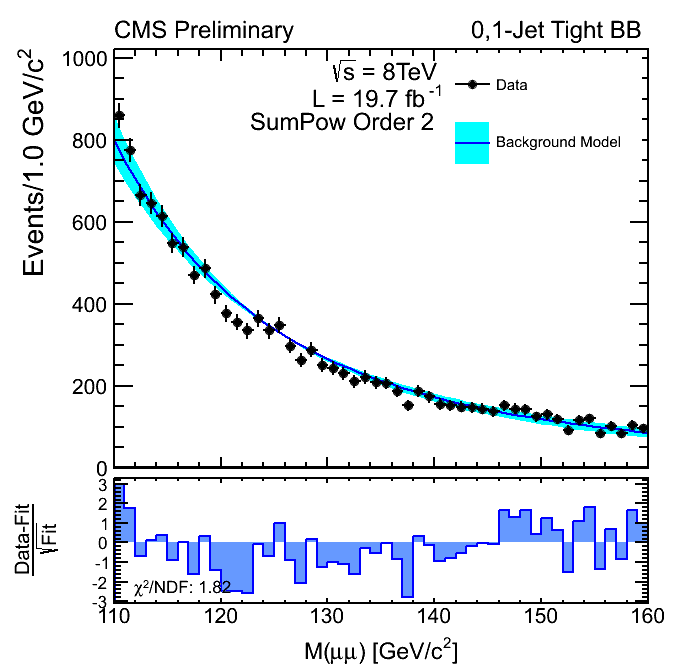
\includegraphics[height=55mm]{2013-10-04SystematicBiasStudy1/order_Shape_Jets01PassPtG10BB_SumPow2}
      \end{center}
   \column{60mm}
      \begin{center}
        $H\rightarrow\gamma\gamma$ AN-13-008 \\
        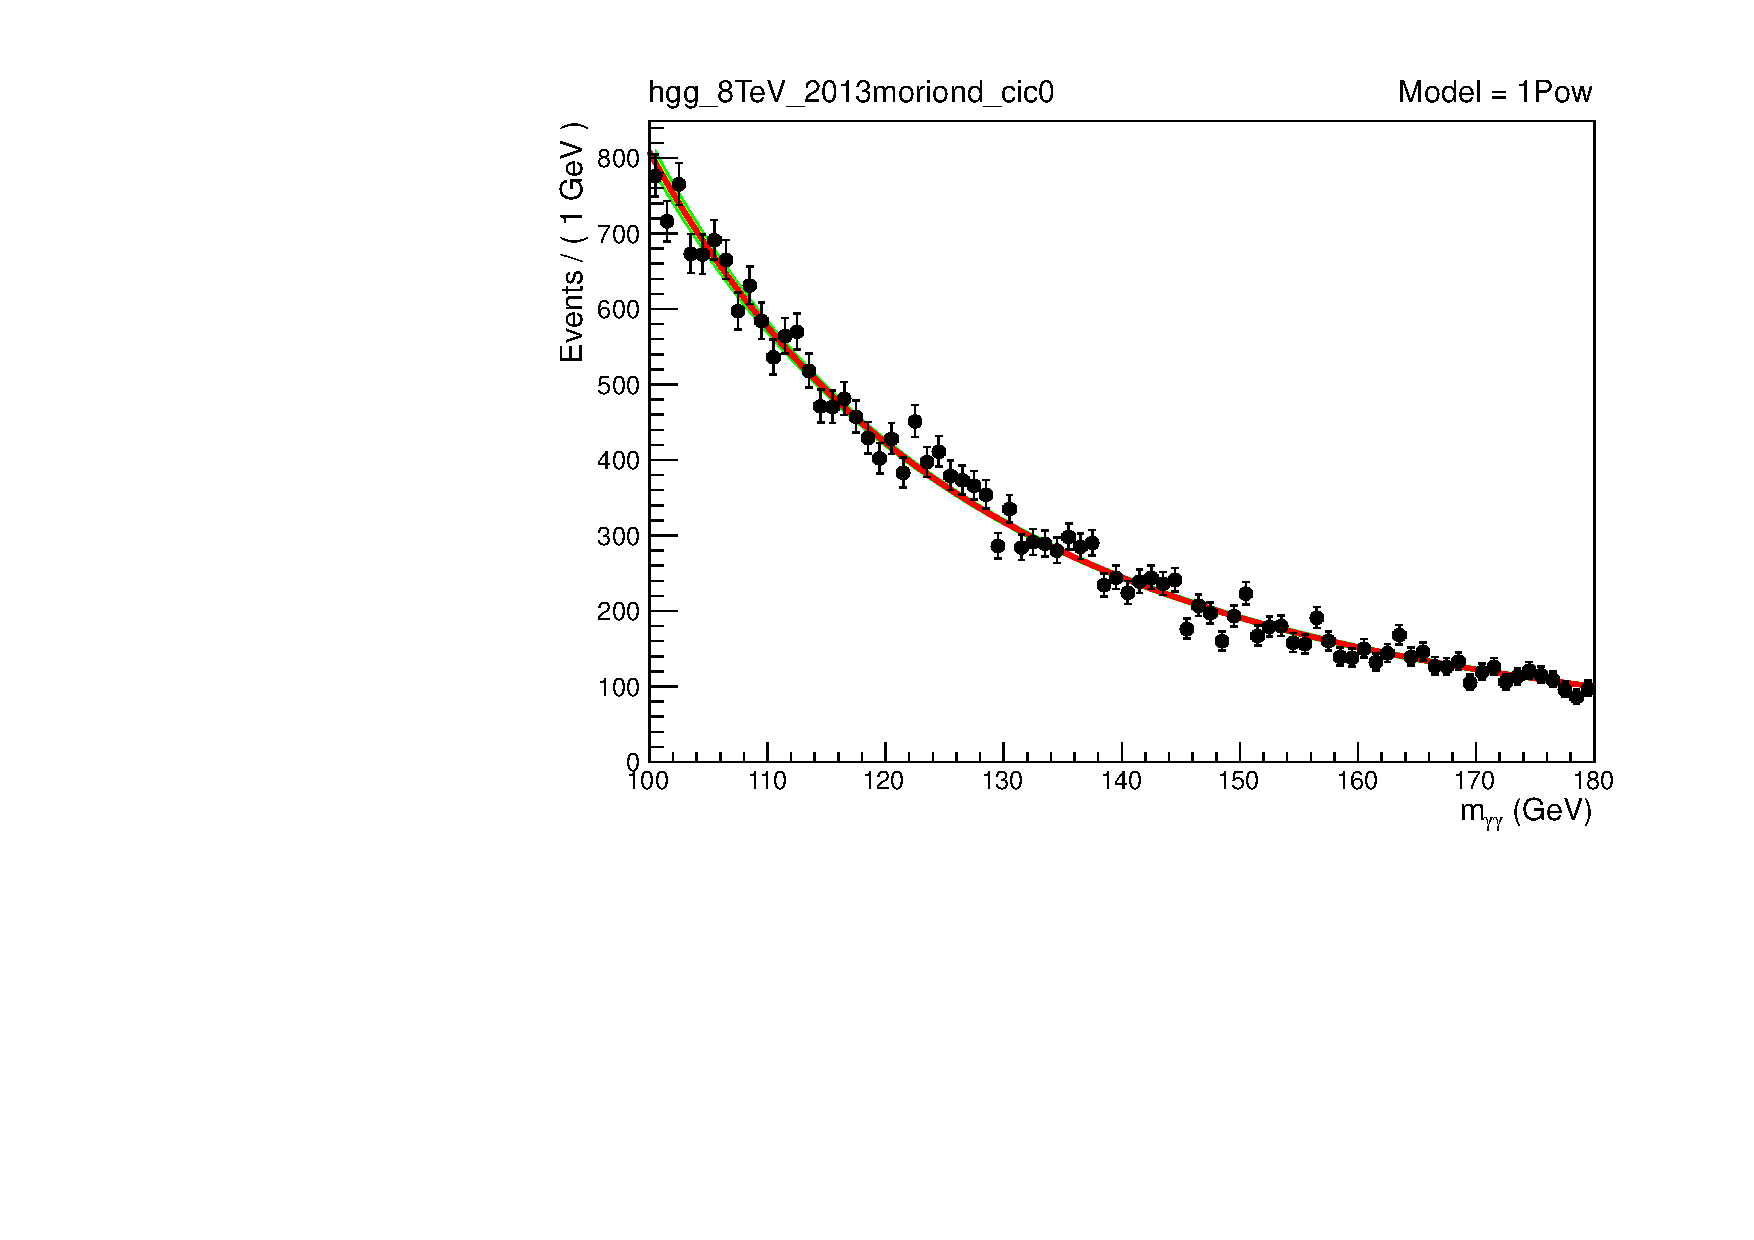
\includegraphics[height=42mm]{2013-10-04SystematicBiasStudy1/truth_hgg_8TeV_2013moriond_cic0_1Pow}
      \end{center}
  \end{columns}
  \begin{center}
    \bf
    \textcolor{red}{
    $H\rightarrow\gamma\gamma$ Shape Much Simpler to Fit
    }
    \\
    $H\rightarrow\mu\mu$ has "Change in Curvature" \& Wider Signal Bump
    \\
    $H\rightarrow\mu\mu$ Requires Higher Orders
  \end{center}
\end{frame}


\begin{frame}
\frametitle{Reference Function Orders Selected}
\vspace{-1em}
\begin{columns}[c]
 \column{60mm}
    \begin{center}
      \textbf{Sum of Exponential \\ Selected Orders }
    \end{center}
    \begin{itemize}
      \item 2-Jet VBF Tight Very Near Threshold to Use 1st Order
      \begin{itemize}
        \item {\scriptsize (Prob: 3\%, Near 5\% Threshold)}
        \item \tred{Decided to Use 1st Order for this Low-Stats Category}
      \end{itemize}
      \item All Other Categories 2nd Order
    \end{itemize}
 \column{60mm}
    \begin{center}
      \textbf{Bernstein Selected Orders}
      \scriptsize
      \begin{tabular}{|l|c|} \hline
                             & Reference       \\
        Category             & Bernstein Order \\ \hline \hline
        0,1-Jet Tight BB     & 4       \\ \hline
        0,1-Jet Tight BO     & 6       \\ \hline
        0,1-Jet Tight BE     & 5       \\ \hline
        0,1-Jet Tight OO     & 4       \\ \hline
        0,1-Jet Tight OE     & 3       \\ \hline
        0,1-Jet Tight EE     & 3       \\ \hline
        0,1-Jet Loose BB     & 4       \\ \hline
        0,1-Jet Loose BO     & 4       \\ \hline
        0,1-Jet Loose BE     & 4       \\ \hline
        0,1-Jet Loose OO     & 4       \\ \hline
        0,1-Jet Loose OE     & 3       \\ \hline
        0,1-Jet Loose EE     & 4       \\ \hline
        2-Jet VBF Tight      & 2       \\ \hline
        2-Jet GF Tight       & 3       \\ \hline
        2-Jet Loose          & 4       \\ \hline
      \end{tabular}
    \small
    \end{center}
\end{columns}
\end{frame}

\begin{frame}
\frametitle{Bernstein Orders Selected by Bias Study}
  \begin{center}
    \scriptsize
    \begin{tabular}{|l|c|c|c|} \hline
                           & Bernstein                & Max Bias w.r.t. & Max Bias w.r.t. \\
Category                  & Selected Order      & Bernstein & SumExp \\ \hline \hline
0,1-Jet Tight BB& 5          &       0.04 &       0.22 \\ \hline
0,1-Jet Tight BO& 6          &       0.00 &       0.15 \\ \hline
0,1-Jet Tight BE& 6          &       0.19 &       0.19 \\ \hline
0,1-Jet Tight OO& 5          &       0.02 &       0.16 \\ \hline
0,1-Jet Tight OE& 5          &       0.03 &       0.07 \\ \hline
0,1-Jet Tight EE& 5          &       0.27 &       0.20 \\ \hline
0,1-Jet Loose BB& 5          &       0.12 &       0.22 \\ \hline
0,1-Jet Loose BO& 5          &       0.15 &       0.15 \\ \hline
0,1-Jet Loose BE& 5          &       0.03 &       0.12 \\ \hline
0,1-Jet Loose OO& 6          &       0.07 &       0.14 \\ \hline
0,1-Jet Loose OE& 5          &       0.05 &       0.13 \\ \hline
0,1-Jet Loose EE& 6          &       0.22 &       0.14 \\ \hline
2-Jet VBF Tight& 2          &       0.00 &       0.09 \\ \hline
2-Jet GF Tight & 5          &       0.21 &       0.27 \\ \hline
2-Jet Loose    & 5          &       0.03 &       0.21 \\ \hline
    \end{tabular}
\\
  \small
    Bias Tested for $m_H \in [120,125,130,135,140,145,150] \GeVcc$
  \end{center}
\end{frame}

\begin{frame}
\frametitle{Combined Bias w.r.t. Bernstein Reference}
  \begin{center}
    \scriptsize
    \begin{tabular}{|l|c|c|c|} \hline
%  Combined Bias w.r.t. Bernstein (Weighted Average)
$m_H$         & Bias & Uncertainty & \\ 
(\GeVcc{})         & ($\sigma/\sigma_{SM}$) & ($\sigma/\sigma_{SM}$) & $\frac{\mathrm{Bias}}{\mathrm{Uncertainty}}$ \\ \hline \hline
115   &      -0.023 &   3.33 &      -0.7\%     \\ \hline
120   &       0.30  &   3.21 &       9.3\%     \\ \hline
125   &       0.15  &   3.10 &       4.8\%     \\ \hline
130   &       0.13  &   3.46 &       3.6\%     \\ \hline
135   &      -0.05  &   4.11 &      -1.1\%     \\ \hline
140   &       0.07  &   5.33 &       1.3\%     \\ \hline
145   &      -0.20  &   7.59 &      -2.6\%     \\ \hline
150   &      -0.54  &  12.6  &      -4.3\%     \\ \hline
155   &      -1.39  &  29.1  &      -4.8\%     \\ \hline
    \end{tabular}
\\ \vspace{1ex}
\normalsize
\textbf{Bernstein w.r.t. Bernstein Bias Small, as Expected}
  \end{center}
  \begin{columns}[c]
     \column{55mm}
    \scriptsize
    \begin{eqnarray*}
      \mu_i &=& \mathrm{Category\,Bias} \\
      \Delta\mu_i &=& \mathrm{Category\,Uncertainty} \\
      w_i &=& 1/(\Delta\mu_i)^2 \\
      w_{tot} &=& \sum w_i \\
    \end{eqnarray*}
     \column{65mm}
        \scriptsize
    \begin{eqnarray*}
      \mu_{\mathrm{Combined}} &=& \frac{1}{w_{tot}} \sum w_i \mu_i \\
      \Delta\mu_{\mathrm{Combined}} &=& \frac{1}{w_{tot}} \sqrt{\sum w_i^2 (\Delta\mu_i)^2} = \frac{1}{\sqrt{w_{tot}}}
    \end{eqnarray*}
  \end{columns}
\end{frame}

\begin{frame}
\frametitle{Combined Bias w.r.t. Sum of Exponential Reference}
  \begin{center}
    \scriptsize
    \begin{tabular}{|l|c|c|c|} \hline
$m_H$         & Bias & Uncertainty & \\ 
(\GeVcc{})         & ($\sigma/\sigma_{SM}$) & ($\sigma/\sigma_{SM}$) & $\frac{\mathrm{Bias}}{\mathrm{Uncertainty}}$ \\ \hline \hline
%  Combined Bias w.r.t. Bernstein (Weighted Average)
115   &      -2.15  &       3.35      &    -64.1\%    \\ \hline
120   &      -0.02  &       3.18      &     -0.7\%    \\ \hline
125   &       0.91  &       3.14      &     28.9\%    \\ \hline
130   &      -0.01  &       3.60      &     -0.3\%    \\ \hline
135   &      -1.13  &       4.36      &    -25.9\%    \\ \hline
140   &      -0.78  &       5.55      &    -13.8\%    \\ \hline
145   &       1.12  &       7.90      &     14.1\%    \\ \hline
150   &       1.60  &      12.3       &     13.1\%    \\ \hline
155   &      -6.22  &      28.0       &    -22.2\%    \\ \hline
    \end{tabular}
\\
  \small
\normalsize
\vspace{1em}
\textbf{Bernstein Bias w.r.t. Sum of Exponentials Large}
\\
Is a Large Biases Expected when Combining many Small Biases?
\\
May need to Require Lower per-Category Biases to Ensure Small Combined Bias
  \end{center}
\end{frame}

\begin{frame}
\frametitle{Expected Limit Comparison $m_H=125\GeVcc{}$}
\begin{center}
\begin{tabular}{|l|c|} \hline
\multicolumn{2}{|c|}{ \bf 0,1-Jet Tight BB Expected Limit for 8 TeV} \\ \hline
\bf Baseline          &      \bf 13.5   \\ \hline
%2th Order Bernstein         & 13.2        \\ \hline
%3th Order Bernstein         & 13.5        \\ \hline
4th Order Bernstein         & 14.5        \\ \hline
5th Order Bernstein         & 14.7        \\ \hline
\bf 6th Order Bernstein         & \tredbf{17.4}        \\ \hline
7th Order Bernstein         & 18.0        \\ \hline
\end{tabular}
\\
All Fitting From 110-160\GeVcc{}
\\ \vspace{1em}
\large
\tredbf{
Performance 30\% Worse
\\
Similar to Adding Extra 80\% Systematic Uncertainty
}
\\
\textbf{Include Uncertainty due to Arbitrary Background Shape}
\end{center}
\end{frame}

%%%%%%%%%%%%%%%%%%%%%%%%%%%%%%%%%%
%%%%%%%%%%%%%%%%%%%%%%%%%%%%%%%%%%
%%%%%%%%%%%%%%%%%%%%%%%%%%%%%%%%%%
%%%%%%%%%%%%%%%%%%%%%%%%%%%%%%%%%%

\begin{frame}
  \begin{center}
    \Huge
    Backup
  \end{center}
\end{frame}

%%%%%%%%%%%%%%%%%%%%%%%%%%%%%%%%%%

\begin{frame}[label=refSelectionMethod]
\frametitle{Reference Function Order Choice Methodology}
  For each Category \& Family, Starting with the Lowest Order, $n$:
\small
  \begin{enumerate}
    \item Perform Unbinned Maximum Likelihood Fits for Order $n$, and for Order $n+1$
    \item Compute the Maximum Likelihood Ratio Statistic:
    \[ \lambda = \frac{\mathcal{L}^{n}(\hat{\theta})}{\mathcal{L}^{n+1}( \hat{\theta}^{'} )}\]
    \item If $n$ is the True Order, $-2\ln\lambda$ is Distributed $\sim \chi^2$ with \\ NDF = Difference in NDF Between Functions of \\ Order $n+1$ and $n$
    \item If $\chi^2$ Probability $\leq5\%$: 
        \\Order $n+1$ is Better than $n$, Repeat Step 1 with Order $n+1$;
        \\ If $\chi^2$ Probability $>5\%$: Keep Order $n$ as Reference
  \end{enumerate}
\end{frame}

\begin{frame}
\frametitle{Families of Reference Models}
\textbf{Sum of Exponentials:}
\\
\[ \mbox{n-Order SumExp}(x) = \sum^n_{i=1}\beta_i e^{\alpha_i x}\]
\\
\hspace{6.5em} NDF = 2$n$
\vspace{1ex}
\\
\textbf{Bernstein Polynomial:}
\[ 
\mbox{n-Order Bernstein}(x) = \sum^n_{i=0}\beta_i 
\left[
\left( \begin{array}{cc}
n \\ i
\end{array} \right)
x^i(1-x)^{n-i}
\right]
\]
\\
\hspace{6.5em} NDF = $n+1$
\\
\begin{center}
\textbf{
Both Used as Reference Function by $\bm{\mathrm{H} \rightarrow \gamma\gamma}$
\\
No Other Appropriate Functions Found
}
\end{center}

\end{frame}

\begin{frame}
\frametitle{Sum of Exponentials: 0,1-Jet Tight BB}
  \begin{columns}[c]
   \column{60mm}
      \begin{center}
      \tiny
\begin{tabular}{|l|c|c|c|c|} \hline
Order & Goodness & $-\ln\mathcal{L}$ & $-2\ln\lambda$ & $p_{\chi^2}$ \\ 
 & of Fit  &  & &  \\ \hline \hline
1 & 1.84e-22 & -51130.74 & 157.66 & 5.83e-35  \\ \hline
\bf 2 & \bf 0.346 & \bf -51051.91 & \bf 0.58 & \bf 0.748  \\ \hline
3 & 0.293 & -51051.62 & 0.82 & 0.665  \\ \hline
4 & 0.26 & -51051.22 & -0.00 & 1  \\ \hline
5 & 0.194 & -51051.22 & -0.00 & 1  \\ \hline
6 & 0.139 & -51051.22 & - & -  \\ \hline
\end{tabular}
\\
\normalsize
\vspace{2em}
\textbf{
Sum of 2 Exponentials Performs well for All Categories}
\\
\vspace{1em}
\tredbf{Not Surprising: Similar Form to Expected Voigtian+Exponential Shape}
      \end{center}
   \column{60mm}
      \begin{center}
        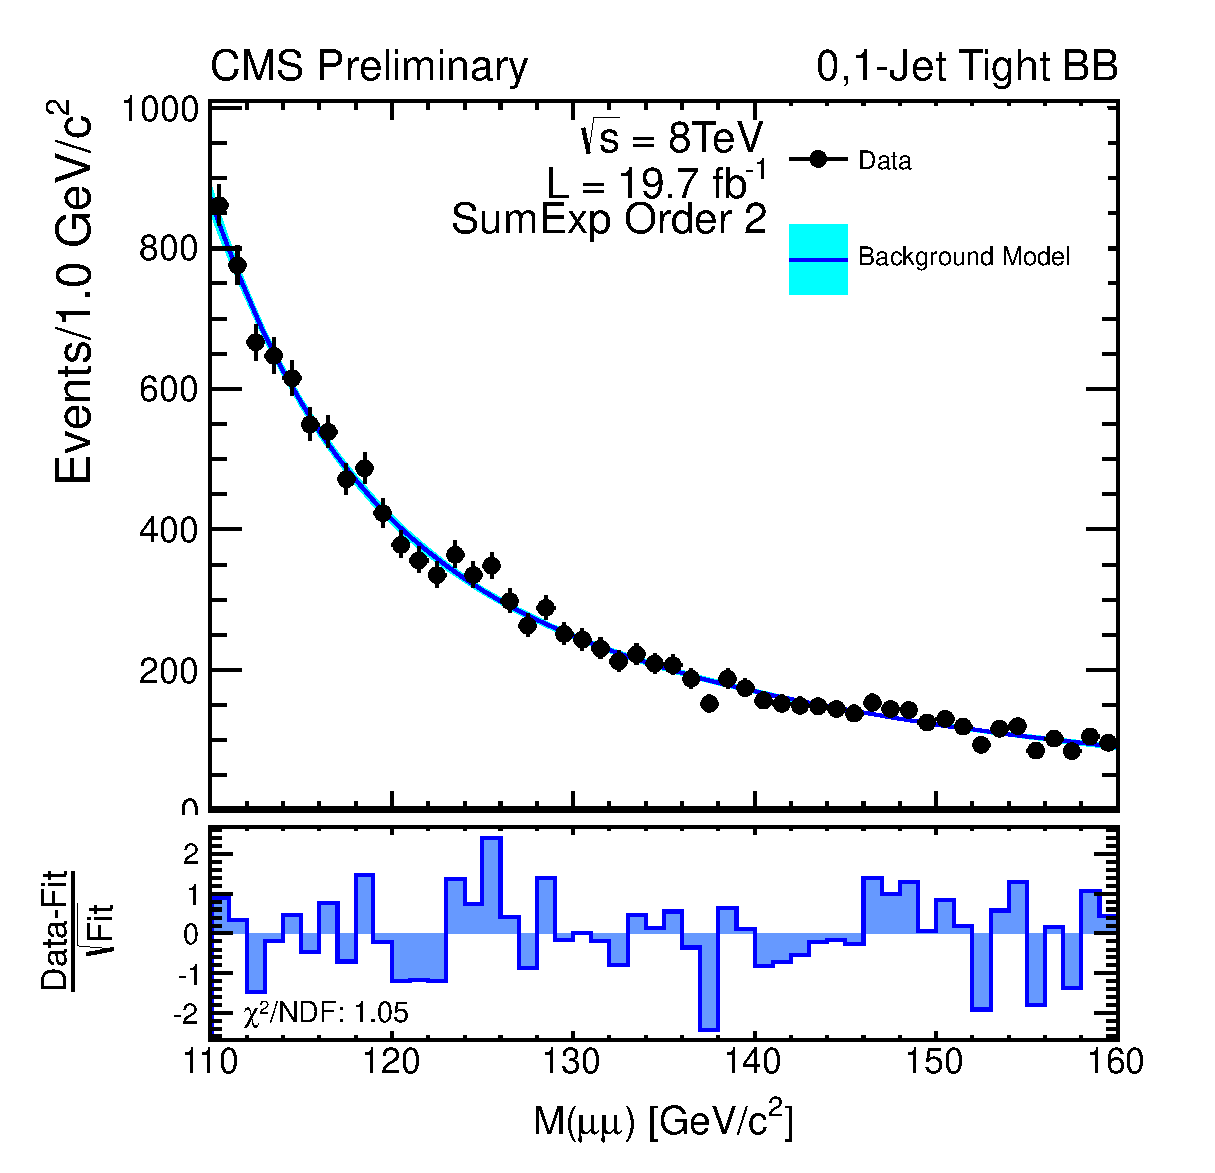
\includegraphics[height=60mm]{wholeRangeHggStudy1/plotsOrderStudyExpPow/order_Shape_Jets01PassPtG10BB_SumExp2}
      \end{center}
  \end{columns}
  \begin{center}
  \end{center}
\end{frame}

\begin{frame}
\frametitle{Bernstein 0,1-Jet Tight BB}
  \begin{columns}[c]
   \column{60mm}
      \begin{center}
      \tiny
\begin{tabular}{|l|c|c|c|c|} \hline
Order & Goodness & $-\ln\mathcal{L}$ & $-2\ln\lambda$ & $p_{\chi^2}$ \\ 
 & of Fit  &  & &  \\ \hline \hline
1 & 2.82e-204 & -51552.21 & 844.80 & 9.81e-186  \\ \hline
2 & 2.51e-22 & -51129.81 & 135.20 & 2.98e-31  \\ \hline
3 & 0.0128 & -51062.21 & 16.62 & 4.57e-05  \\ \hline
\bf 4 & \bf 0.162 & \bf -51053.90 & \bf 2.51 & \bf 0.113  \\ \hline
5 & 0.196 & -51052.65 & 4.92 & 0.0265  \\ \hline
6 & 0.332 & -51050.19 & 1.61 & 0.205  \\ \hline
7 & 0.368 & -51049.38 & 0.10 & 0.75  \\ \hline
8 & 0.338 & -51049.33 & 0.38 & 0.535  \\ \hline
9 & 0.302 & -51049.14 & - & -  \\ \hline
\end{tabular}
\\
\normalsize
\vspace{2em}
\bf
Most Categories Similar
\\
Tight BO \& BE Require Higher Order
      \end{center}
   \column{60mm}
      \begin{center}
        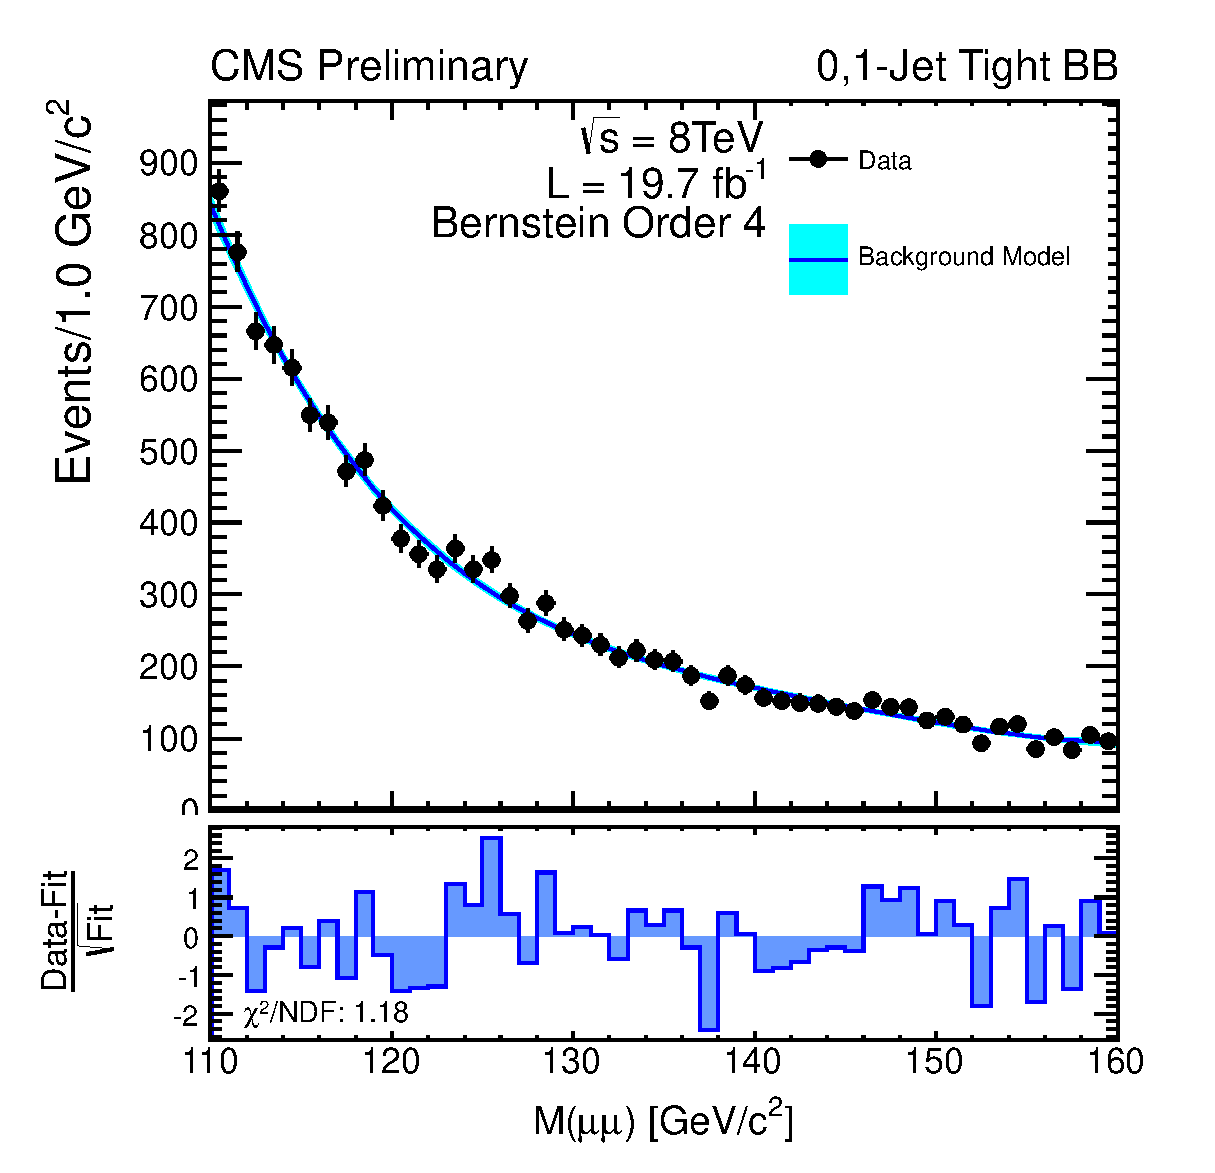
\includegraphics[height=55mm]{wholeRangeHggStudy1/plotsOrderStudyPolysLowOrders/order_Shape_Jets01PassPtG10BB_Bernstein4}
      \end{center}
  \end{columns}
  \begin{center}
  \end{center}
\end{frame}

\begin{frame}
\frametitle{Bernstein 0,1-Jet Tight BO}
  \begin{columns}[c]
   \column{60mm}
      \begin{center}
      \tiny
\begin{tabular}{|l|c|c|c|c|} \hline
Order & Goodness & $-\ln\mathcal{L}$ & $-2\ln\lambda$ & $p_{\chi^2}$ \\ 
 & of Fit  &  & &  \\ \hline \hline
1 & 0 & -89577.79 & 1266.13 & 2.59e-277  \\ \hline
2 & 4.43e-40 & -88944.72 & 222.67 & 2.37e-50  \\ \hline
3 & 0.00147 & -88833.39 & 21.74 & 3.12e-06  \\ \hline
4 & 0.079 & -88822.52 & 17.11 & 3.53e-05  \\ \hline
5 & 0.579 & -88813.97 & 8.08 & 0.00447  \\ \hline
\bf 6 & \bf 0.796 & \bf -88809.92 & \bf 1.84 & \bf 0.175  \\ \hline
7 & 0.785 & -88809.00 & -0.22 & 1  \\ \hline
8 & 0.732 & -88809.12 & 0.46 & 0.496  \\ \hline
9 & 0.72 & -88808.88 & - & -  \\ \hline
\end{tabular}
\\
\normalsize
\vspace{2em}
\tredbf{Must Fit 6 Parameters For Background Shape}
      \end{center}
   \column{60mm}
      \begin{center}
        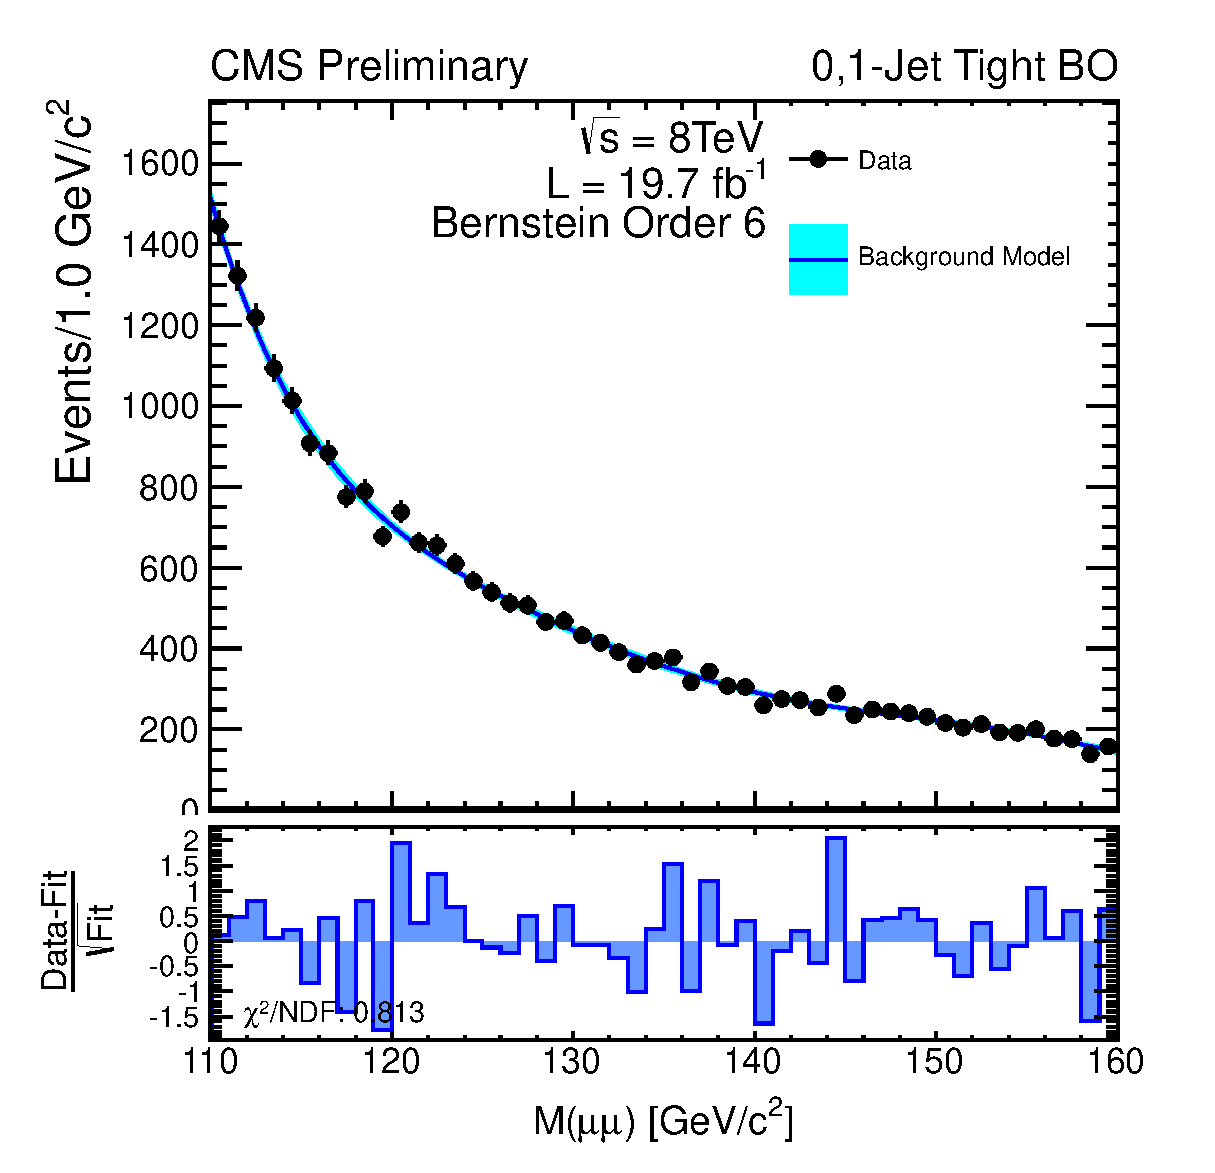
\includegraphics[height=55mm]{wholeRangeHggStudy1/plotsOrderStudyPolysHighOrders/order_Shape_Jets01PassPtG10BO_Bernstein6}
      \end{center}
  \end{columns}
  \begin{center}
  \end{center}
\end{frame}

\begin{frame}[label=biasEstimateMethod]
\frametitle{Bias Estimate Methodology}
  For Each Reference Background Model, and Alternate Model to be Tested:
  \begin{itemize}
    \item Fit Reference to 8 TeV Data
    \item Generate 1000 Toy Datasets from Reference Model
    \item For each Toy Dataset:
    \begin{itemize}
        \item Re-fit with Signal+Reference Background Model
        \item Fit with Signal+Alternate Background Model
        \item Compute $R = \frac{N_{sig}(Alt)-N_{sig}(Ref)}{\Delta N_{sig}(Alt)}$
            \\ where $N_{sig}$ is the amount of signal estimated in the fit
            \\ and $\Delta N_{sig}$ is the uncertainty from the fit
    \end{itemize}
    \item $R$ Estimates Amount of Bias w.r.t. Statistical Uncertainty
  \end{itemize}
\end{frame}

\begin{frame}
\frametitle{Bias Study Results: 0,1-Jet Tight BB}
\scriptsize
\begin{center}
\begin{tabular}{|l|r|r|} \hline 
\multicolumn{3}{|c|}{ \bf 0,1-Jet Tight BB Maximum Bias} \\ \hline
\multicolumn{1}{|c|}{\multirow{3}{*}{Alternate PDFs}} & \multicolumn{2}{c|}{Reference PDFs} \\ \cline{2-3} 
& \multicolumn{1}{c|}{4th-Order} & \multicolumn{1}{c|}{2nd-Order} \\ 
& \multicolumn{1}{c|}{      Bernstein} & \multicolumn{1}{c|}{Sum of Exponentials} \\ \hline
4th-Order Bernstein &           -0.1\% &           79.6\% \\ \hline
5th-Order Bernstein &           -5.0\% &          -32.0\% \\ \hline
\textbf{6th-Order Bernstein} &            \textbf{3.5\%} &          \textbf{-14.2\%} \\ \hline
7th-Order Bernstein &           -4.2\% &          -12.2\% \\ \hline
8th-Order Bernstein &            6.4\% &          -11.9\% \\ \hline
9th-Order Bernstein &            8.0\% &          -14.1\% \\ \hline
\end{tabular}
\small
\\ \vspace{1em}
Maximum Bias for $m_H:$ [115,120,125,135,150,155] \GeVcc{}
\\
\bf
4th-Order Bernstein Works Well
\end{center}
\end{frame}

\begin{frame}
\frametitle{Bias Study Results: 0,1-Jet Tight BO}
\scriptsize
\begin{center}
\begin{tabular}{|l|r|r|} \hline 
\multicolumn{3}{|c|}{ \bf 0,1-Jet Tight BO Maximum Bias} \\ \hline
\multicolumn{1}{|c|}{\multirow{3}{*}{Alternate PDFs}} & \multicolumn{2}{c|}{Reference PDFs} \\ \cline{2-3} 
& \multicolumn{1}{c|}{6th-Order} & \multicolumn{1}{c|}{2nd-Order} \\ 
& \multicolumn{1}{c|}{      Bernstein} & \multicolumn{1}{c|}{Sum of Exponentials} \\ \hline
4th-Order Bernstein &          255.8\% &         -150.7\% \\ \hline
5th-Order Bernstein &         -107.4\% &          -71.2\% \\ \hline
\textbf{6th-Order Bernstein} &           \textbf{-0.0\%} &          \tredbf{-25.9\%} \\ \hline
7th-Order Bernstein &           34.0\% &          -12.8\% \\ \hline
8th-Order Bernstein &           31.0\% &          -10.2\% \\ \hline
9th-Order Bernstein &           35.9\% &           -9.9\% \\ \hline
\end{tabular}
\small
\\ \vspace{1em}
Maximum Bias for $m_H:$ [115,120,125,135,150,155] \GeVcc{}
\\
\tredbf{
Problems with Large Bias for High-Order Bernstein
%\\ $\bm{\sim 30\%}$ Best Bias for BE
%\\ Other Categories May Have Higher Biases
\\ Currently Investigating Other Categories \& Wider Fit Range
}
\end{center}
\end{frame}


\begin{frame}
\frametitle{Investigating $\Delta N_{sig}$ Estimates with ``Pulls''}
\begin{columns}[c]
 \column{60mm}
  \small
  \begin{itemize}
    \item Are Fit Errors Calculated Properly?
    \item ``Pull'' Sometimes too Wide: \\$\Delta N_{sig}$ Under-Estimated
    \item \tredbf{Causes Bias Over-Estimates}
    \item \tredbf{May Cause Coverage Problems}
  \end{itemize}
  \begin{center}
    \tiny
    \begin{tabular}{|l|c|c|c|c|} \hline 
    \multicolumn{5}{|c|}{\bf 0,1-Jet Tight BB} \\ \hline
    \bf Order &  \bf 1-5 &\bf  6,7 &\bf  8 &\bf  9 \\ \hline
    Bernstein $\sigma_{Pull}$ & $\sim0\%$ & $\sim10\%$ & $\sim20\%$ & $\sim30\%$ \\ \hline
    %\hline
    %\bf Order & \multicolumn{2}{c|}{\bf 1,2} & \multicolumn{2}{c|}{\bf $\geq3$} \\ \hline
    %SumExp $\sigma_{Pull}$ & \multicolumn{2}{c|}{$<3\%$} & \multicolumn{2}{c|}{$\geq50\%$} \\ \hline
    \end{tabular}
  \end{center}
 \column{60mm}
    \begin{center}
      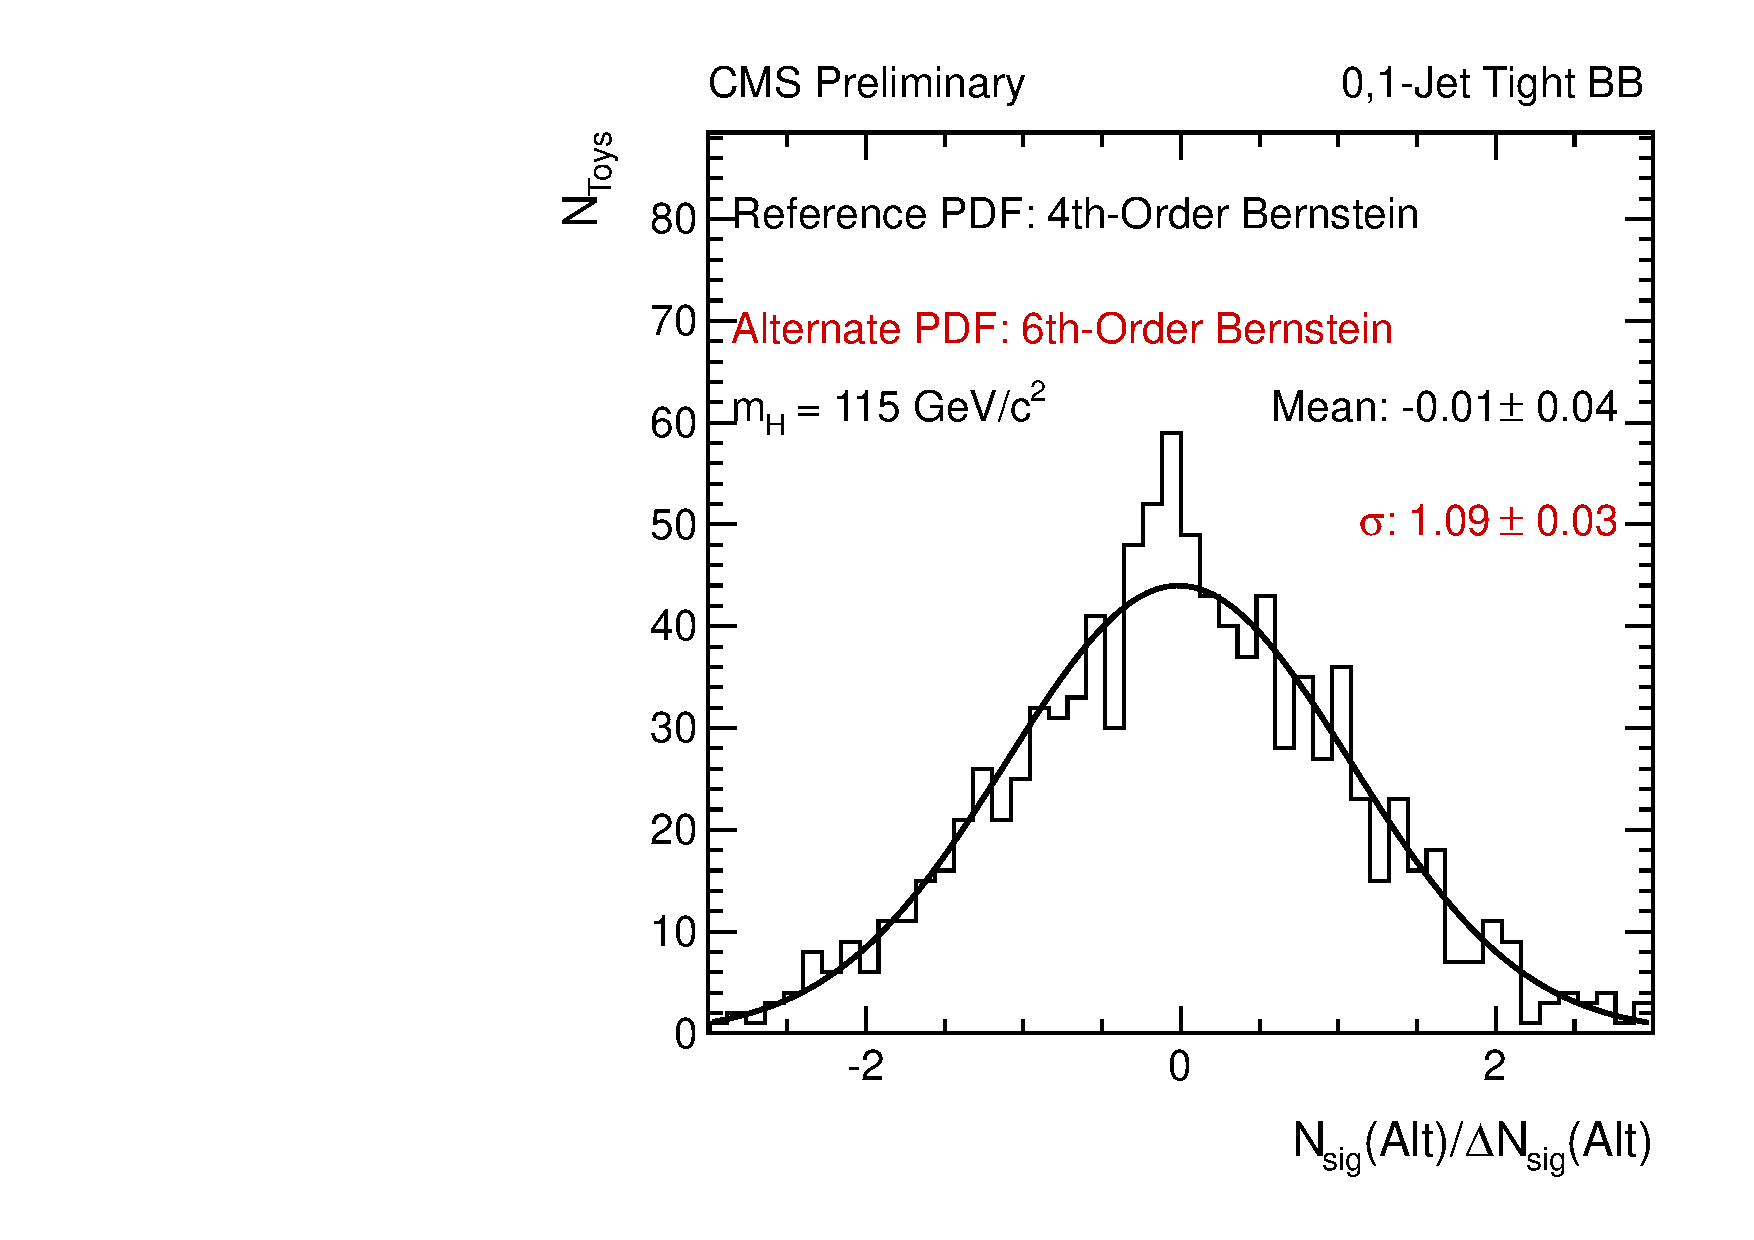
\includegraphics[height=55mm]{redoWholeRange/biasStudy/bias_Jets01PassPtG10BB_115_Z_RefBernstein_Alt6Bernstein.pdf}
      %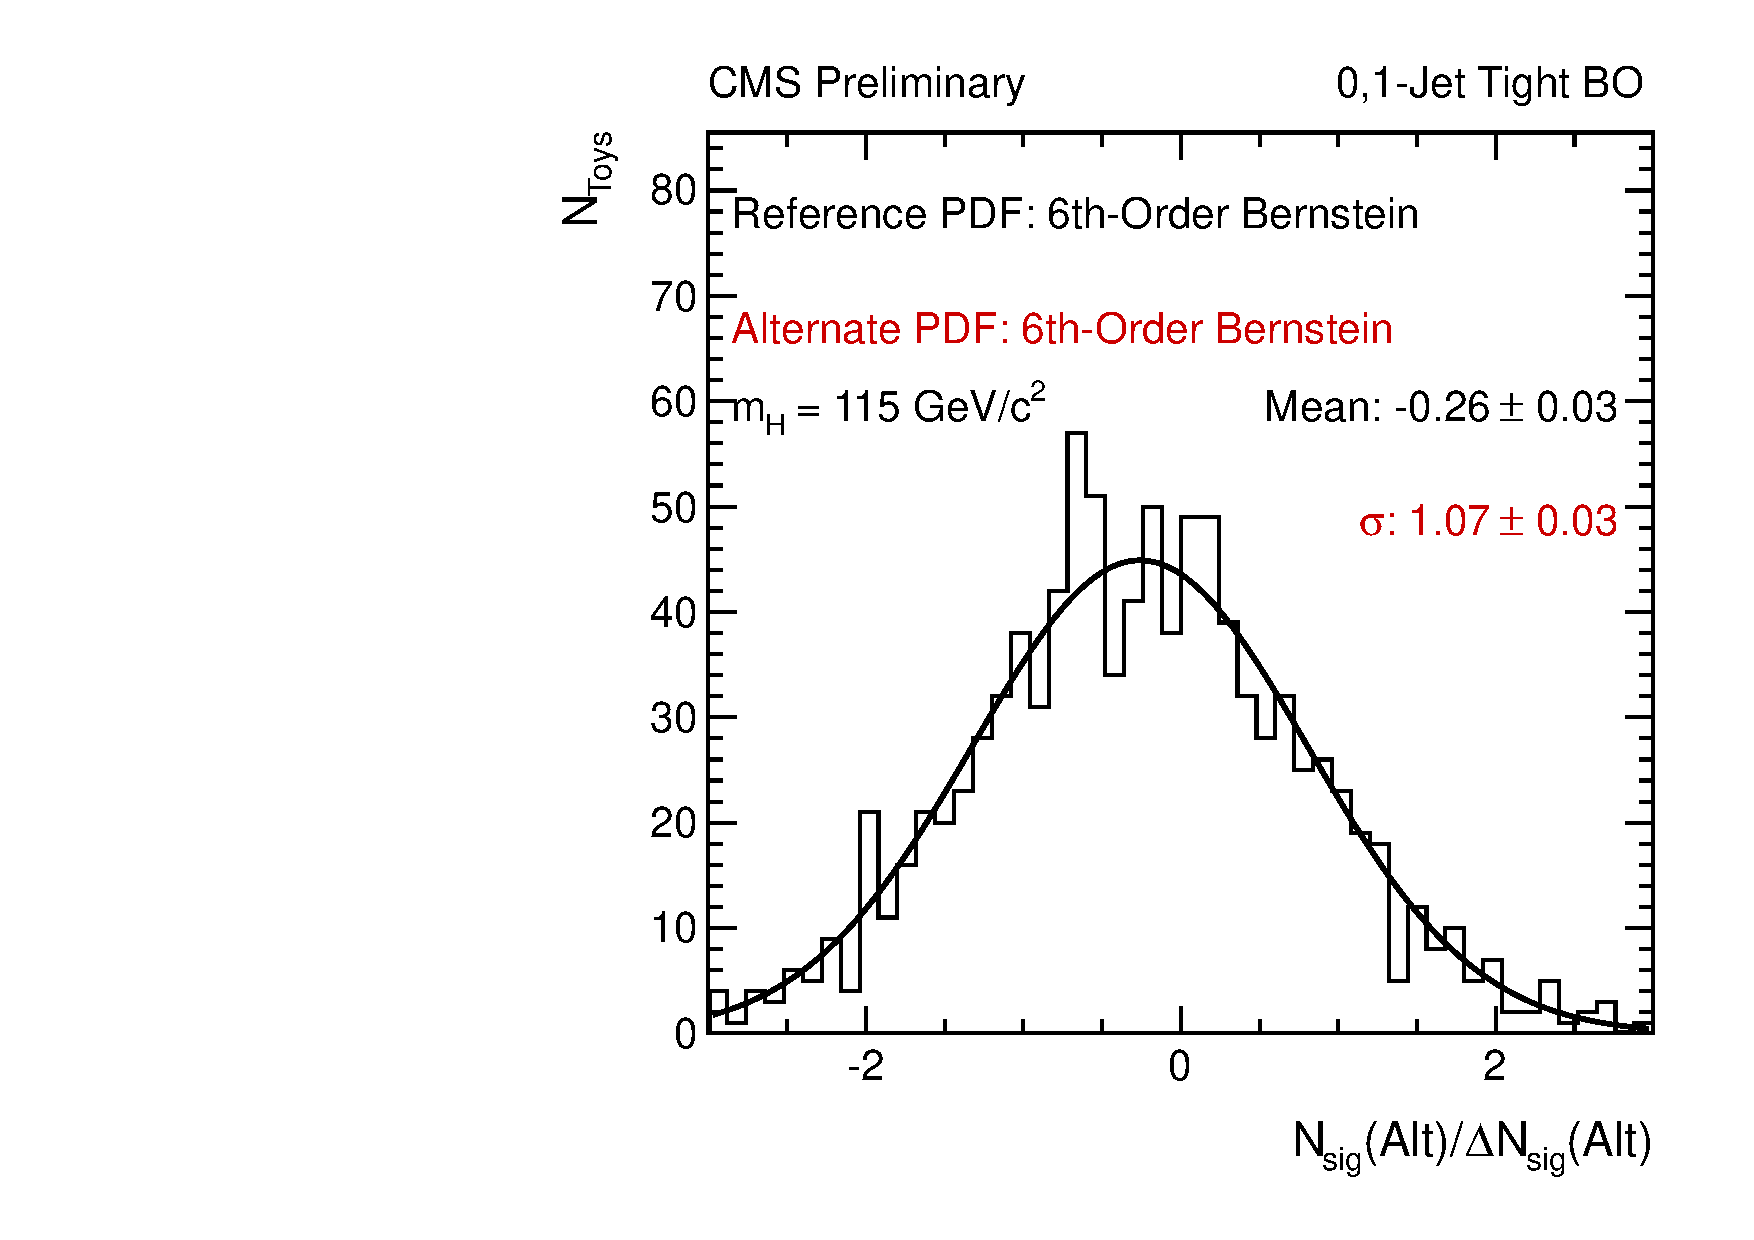
\includegraphics[height=55mm]{redoWholeRange/biasStudy/bias_Jets01PassPtG10BO_115_Z_RefBernstein_Alt6Bernstein.pdf}
    \end{center}
\end{columns}
\begin{center}
  \large
  \tredbf{
  For now, Move on, Calculate Performance
  }
\end{center}
\end{frame}


\begin{frame}
\frametitle{Baseline 0,1-Jet Tight BB/BO Fits}
  \vspace{-1em}
  \begin{columns}[c]
   \column{60mm}
      \begin{center}
        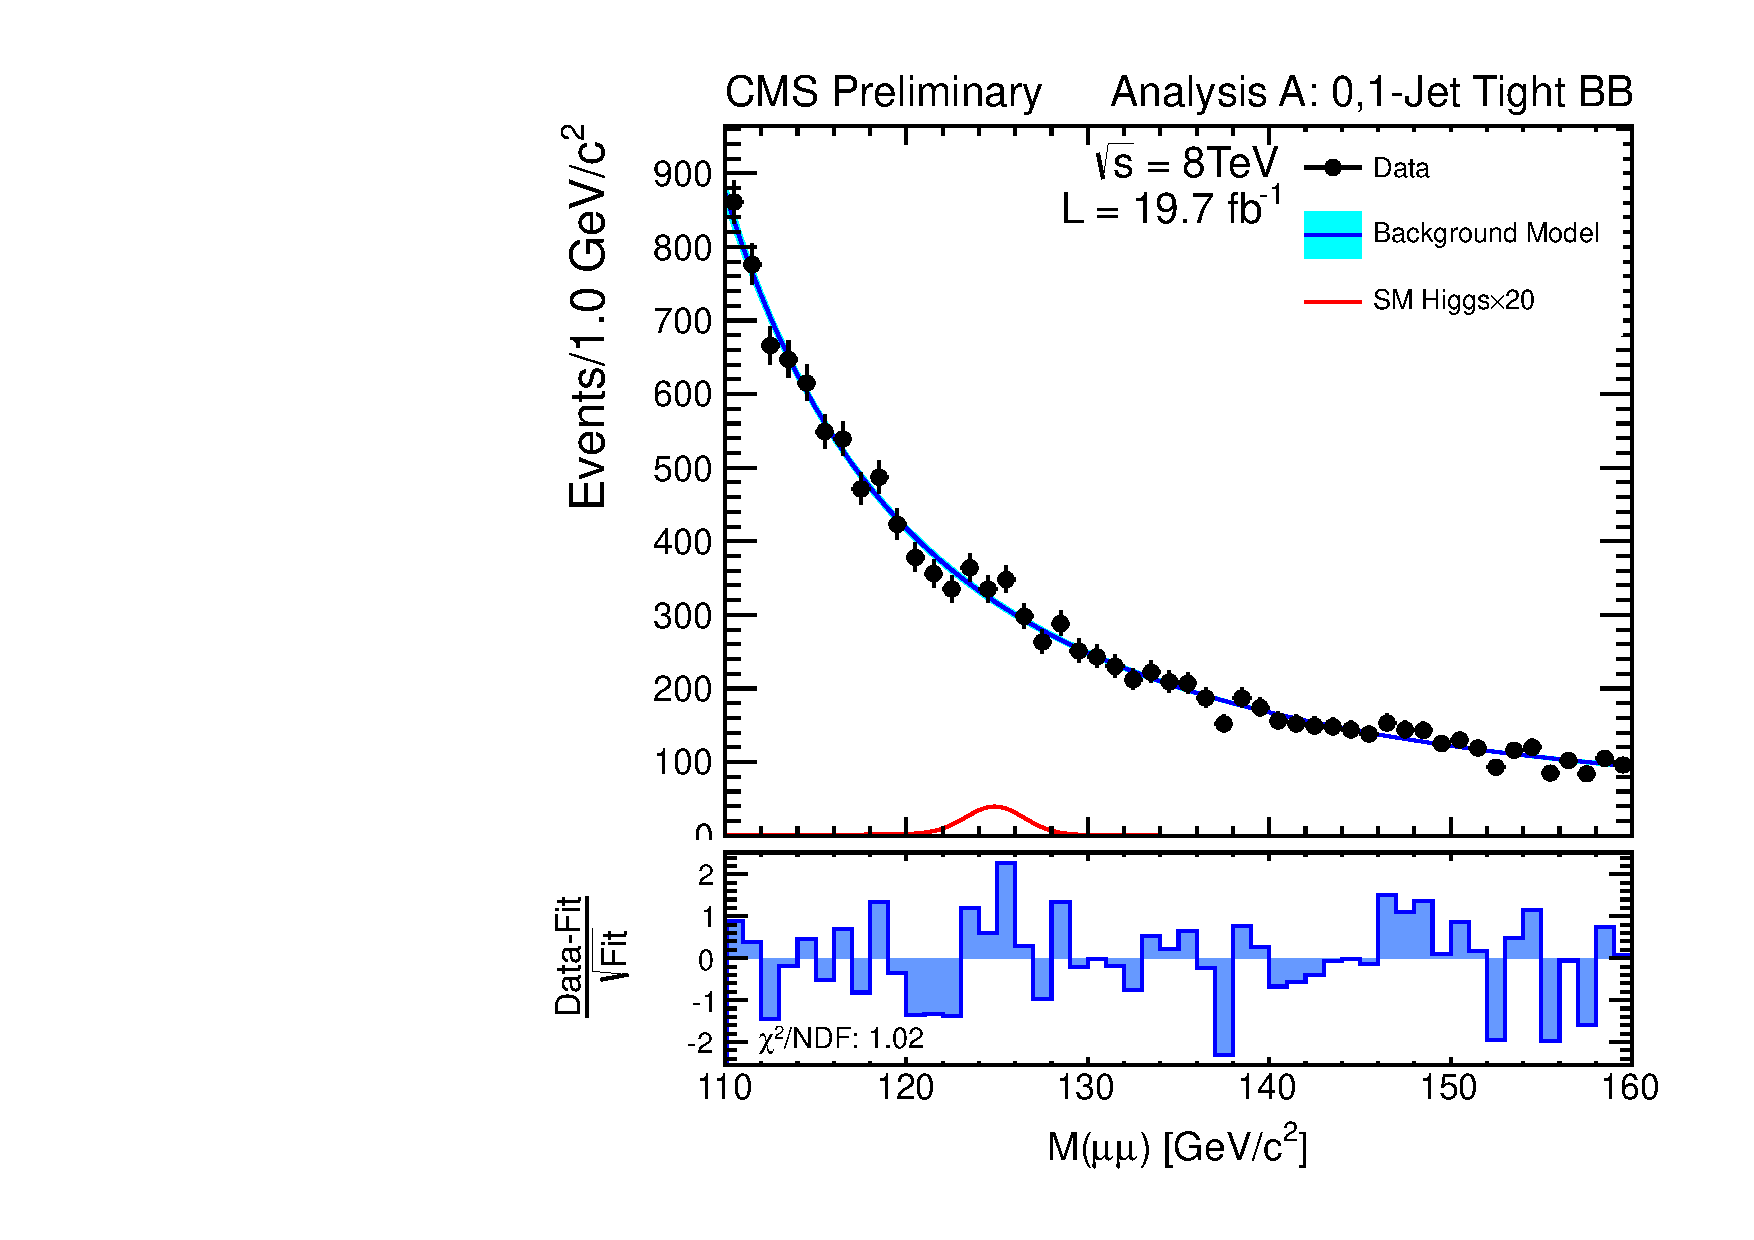
\includegraphics[height=60mm]{plotsPublic/mass_AnanlysisA/pdf/CombSplitAll_8TeV_125_Jets01PassPtG10BB.pdf}
      \end{center}
   \column{60mm}
      \begin{center}
        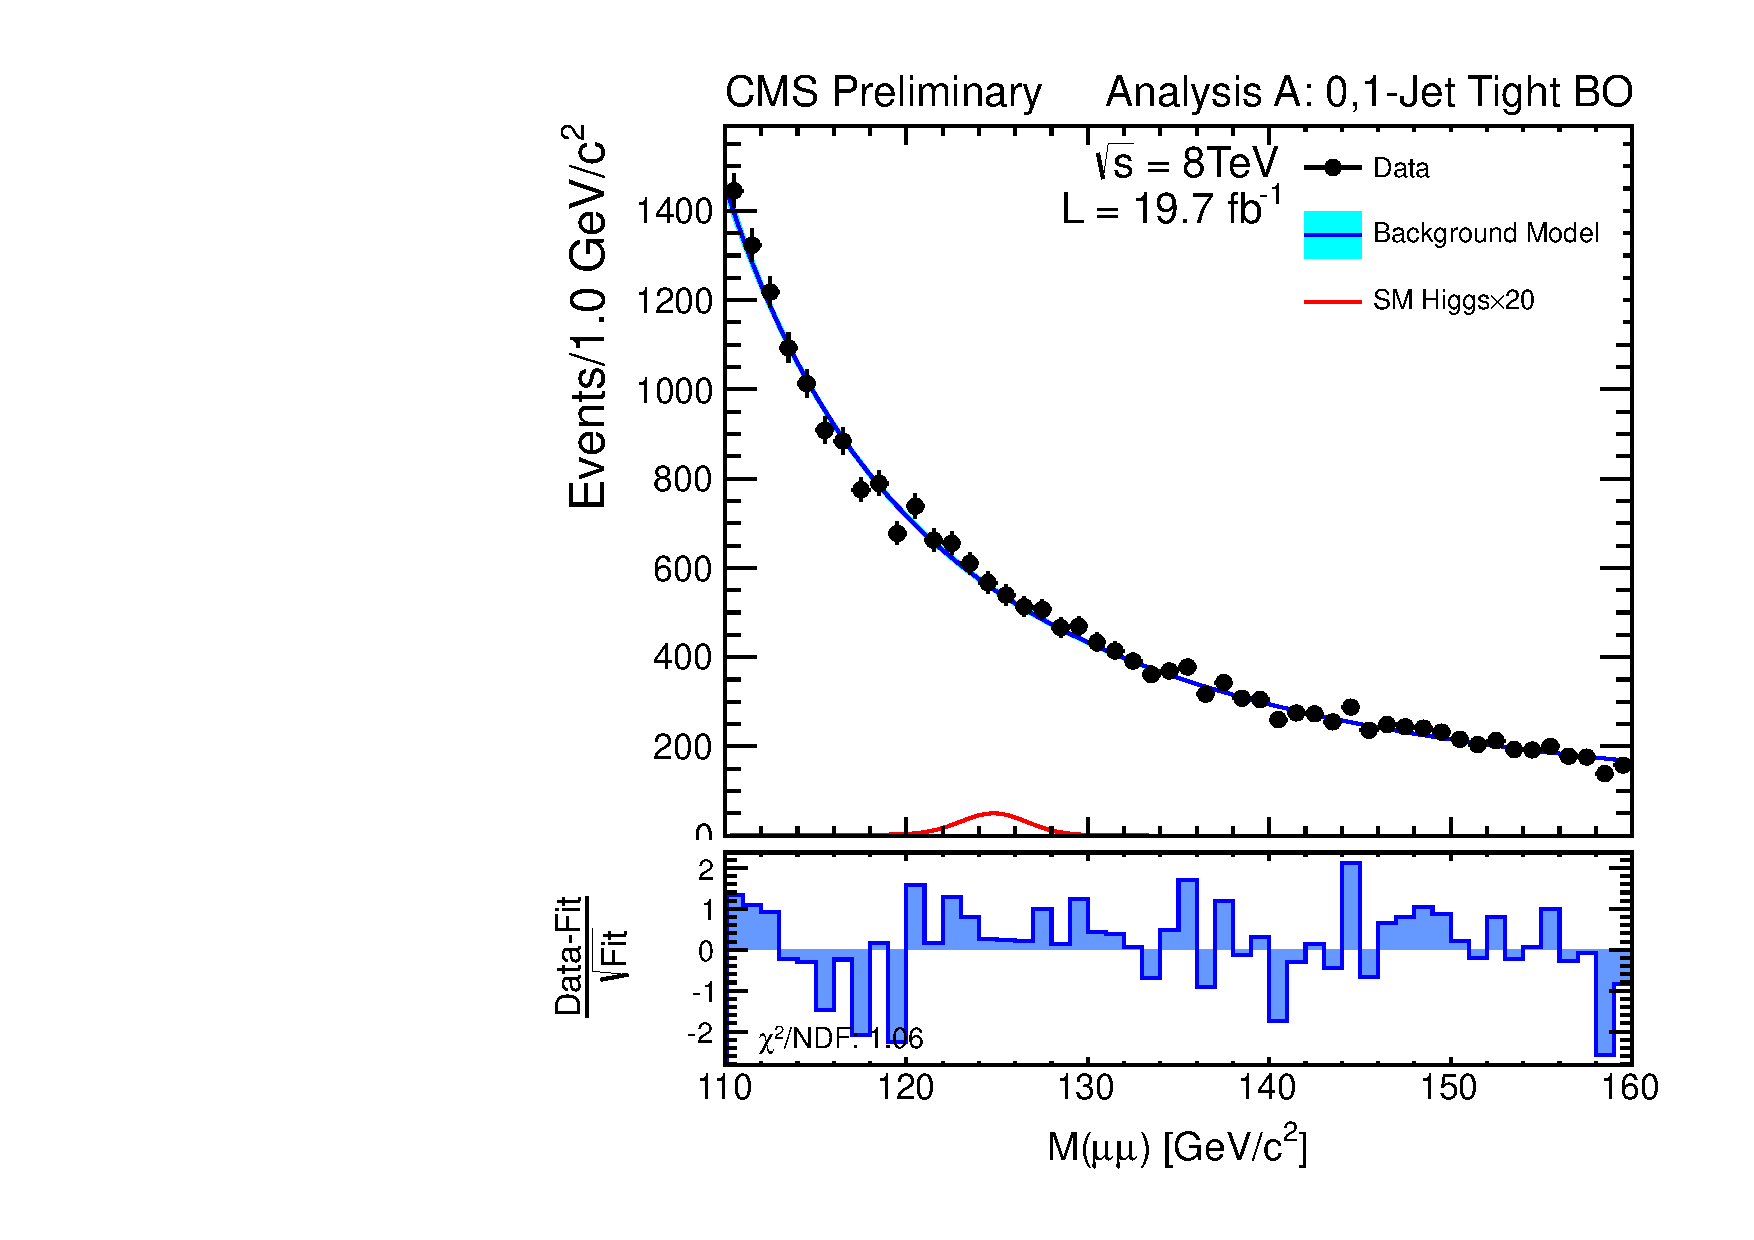
\includegraphics[height=60mm]{plotsPublic/mass_AnanlysisA/pdf/CombSplitAll_8TeV_125_Jets01PassPtG10BO.pdf}
      \end{center}
  \end{columns}
\begin{center}
\end{center}
\end{frame}


\begin{frame}
\frametitle{Sum of Exponentials 0,1-Jet Tight BO}
  \begin{columns}[c]
   \column{60mm}
      \begin{center}
      \tiny
\begin{tabular}{|l|c|c|c|c|} \hline
Order & Goodness & $-\ln\mathcal{L}$ & $-2\ln\lambda$ & $p_{\chi^2}$ \\ 
 & of Fit  &  & &  \\ \hline \hline
1 & 7.59e-37 & -88937.36 & 245.23 & 5.6e-54  \\ \hline
\bf 2 & \bf 0.577 & \bf -88814.74 & \bf 4.83 & \bf 0.0895  \\ \hline
3 & 0.63 & -88812.33 & 0.11 & 0.949  \\ \hline
4 & 0.548 & -88812.28 & 0.74 & 0.69  \\ \hline
5 & 0.485 & -88811.91 & -1.39 & 1  \\ \hline
6 & 0.346 & -88812.60 & - & -  \\ \hline
\end{tabular}
      \end{center}
   \column{60mm}
      \begin{center}
        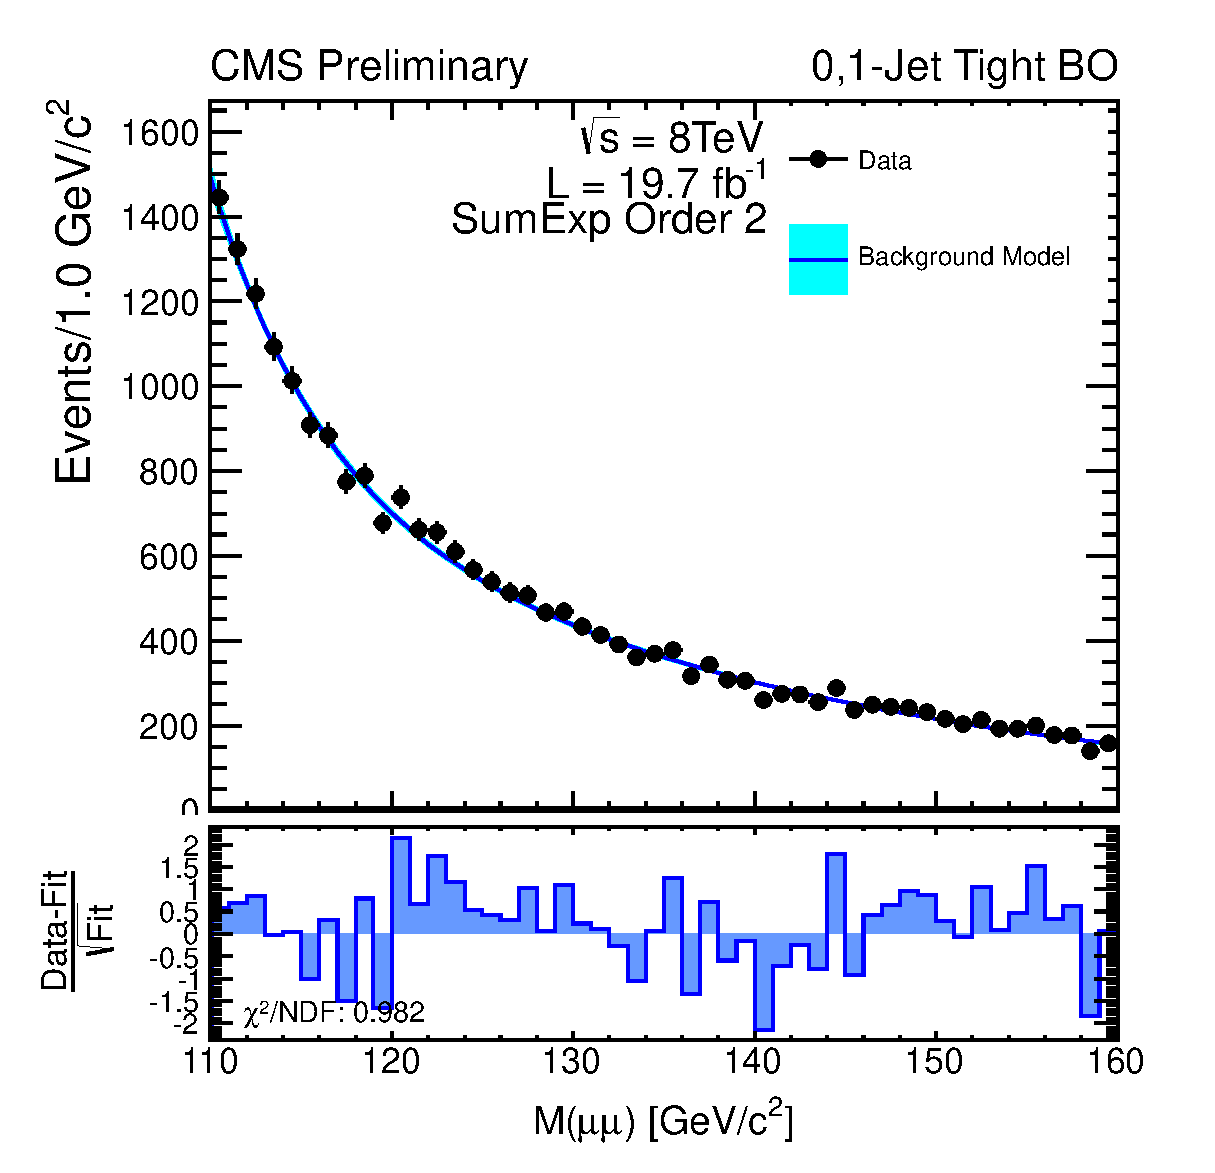
\includegraphics[height=55mm]{wholeRangeHggStudy1/plotsOrderStudyExpPow/order_Shape_Jets01PassPtG10BO_SumExp2}
      \end{center}
  \end{columns}
  \begin{center}
  \end{center}
\end{frame}

\begin{frame}
\frametitle{Sum of Exponentials 0,1-Jet Tight BE}
  \begin{columns}[c]
   \column{60mm}
      \begin{center}
      \tiny
\begin{tabular}{|l|c|c|c|c|} \hline
Order & Goodness & $-\ln\mathcal{L}$ & $-2\ln\lambda$ & $p_{\chi^2}$ \\ 
 & of Fit  &  & &  \\ \hline \hline
1 & 8.86e-130 & -40641.90 & 550.30 & 1.08e-121  \\ \hline
2 & 2.93e-14 & -40366.75 & 78.28 & 8.96e-19  \\ \hline
3 & 0.000671 & -40327.61 & 14.38 & 0.000149  \\ \hline
4 & 0.0137 & -40320.42 & 7.27 & 0.007  \\ \hline
\bf 5 & \bf 0.0359 & \bf -40316.78 & \bf 0.40 & \bf 0.526  \\ \hline
6 & 0.0299 & -40316.58 & 1.72 & 0.19  \\ \hline
7 & 0.0286 & -40315.73 & 0.54 & 0.464  \\ \hline
8 & 0.0211 & -40315.46 & 0.56 & 0.453  \\ \hline
9 & 0.0177 & -40315.18 & - & -  \\ \hline
\end{tabular}
      \end{center}
   \column{60mm}
      \begin{center}
        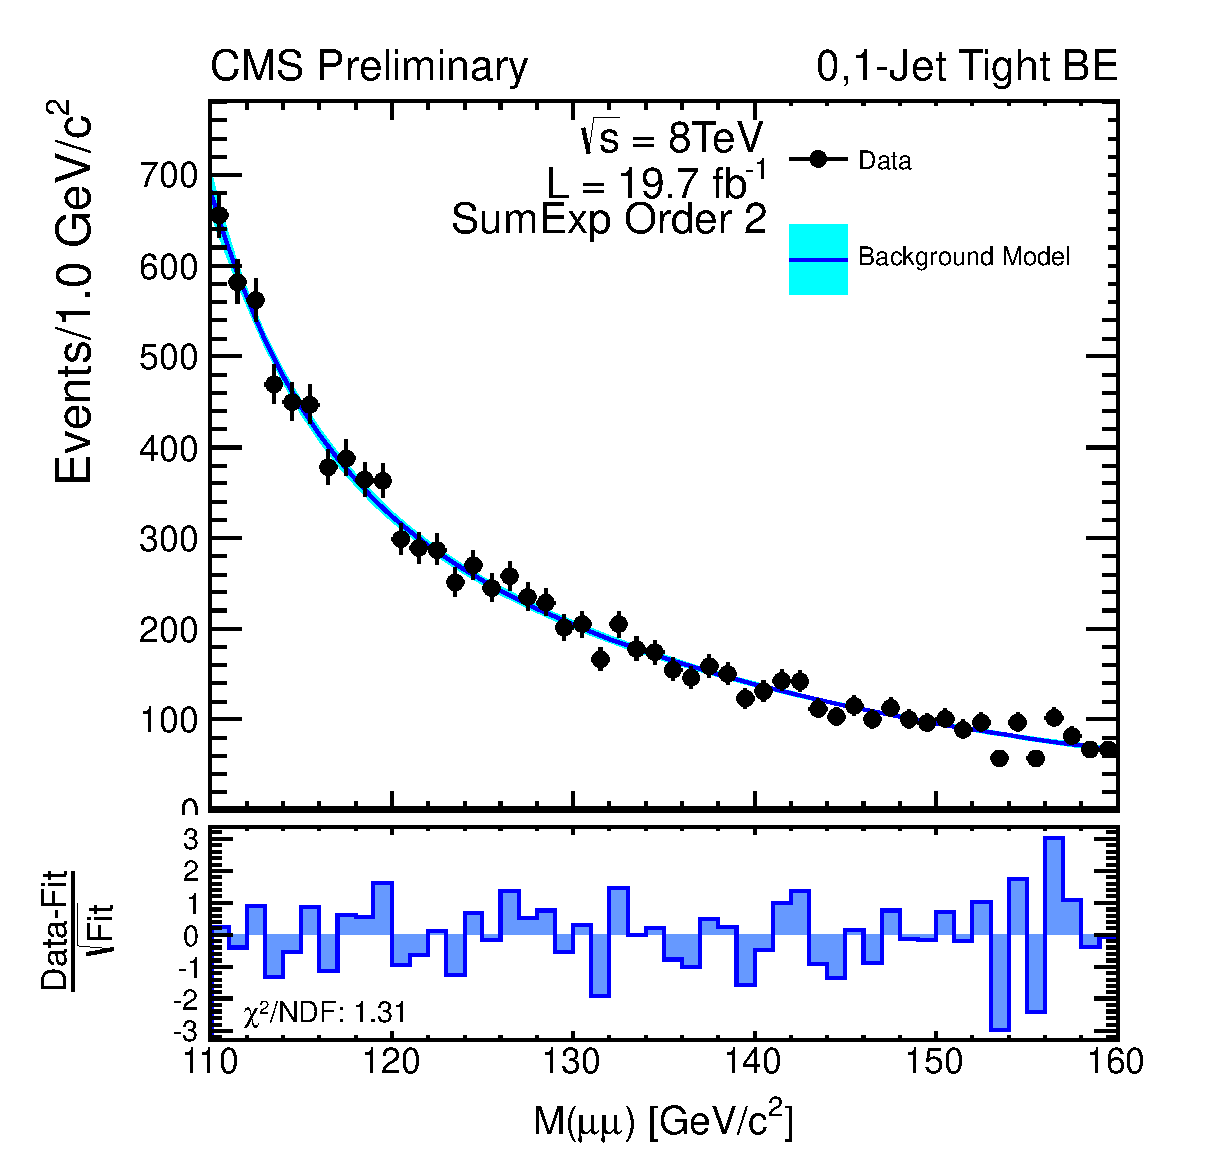
\includegraphics[height=55mm]{wholeRangeHggStudy1/plotsOrderStudyExpPow/order_Shape_Jets01PassPtG10BE_SumExp2}
      \end{center}
  \end{columns}
  \begin{center}
  \end{center}
\end{frame}


\begin{frame}
\frametitle{Sum of Exponentials 2-Jet Tight VBF}
  \begin{columns}[c]
   \column{60mm}
      \begin{center}
      \tiny
\begin{tabular}{|l|c|c|c|c|} \hline
Order & Goodness & $-\ln\mathcal{L}$ & $-2\ln\lambda$ & $p_{\chi^2}$ \\ 
 & of Fit  &  & &  \\ \hline \hline
1 & 0.439 & -344.44 & 6.98 & 0.0305  \\ \hline
\bf 2 & \bf 0.8 & \bf -340.95 & \bf 0.00 & \bf 1  \\ \hline
3 & 0.734 & -340.95 & -0.00 & 1  \\ \hline
4 & 0.656 & -340.95 & 0.58 & 0.749  \\ \hline
5 & 0.573 & -340.66 & 0.04 & 0.981  \\ \hline
6 & 0.48 & -340.64 & - & -  \\ \hline
\end{tabular}
\\
\normalsize
\vspace{2em}
\bf
Sum of 2 Exponentials Performs well for All Categories
\\
\vspace{1em}
Not surprising: Similar Form to Expected Voigtian+Exponential Shape
      \end{center}
   \column{60mm}
      \begin{center}
        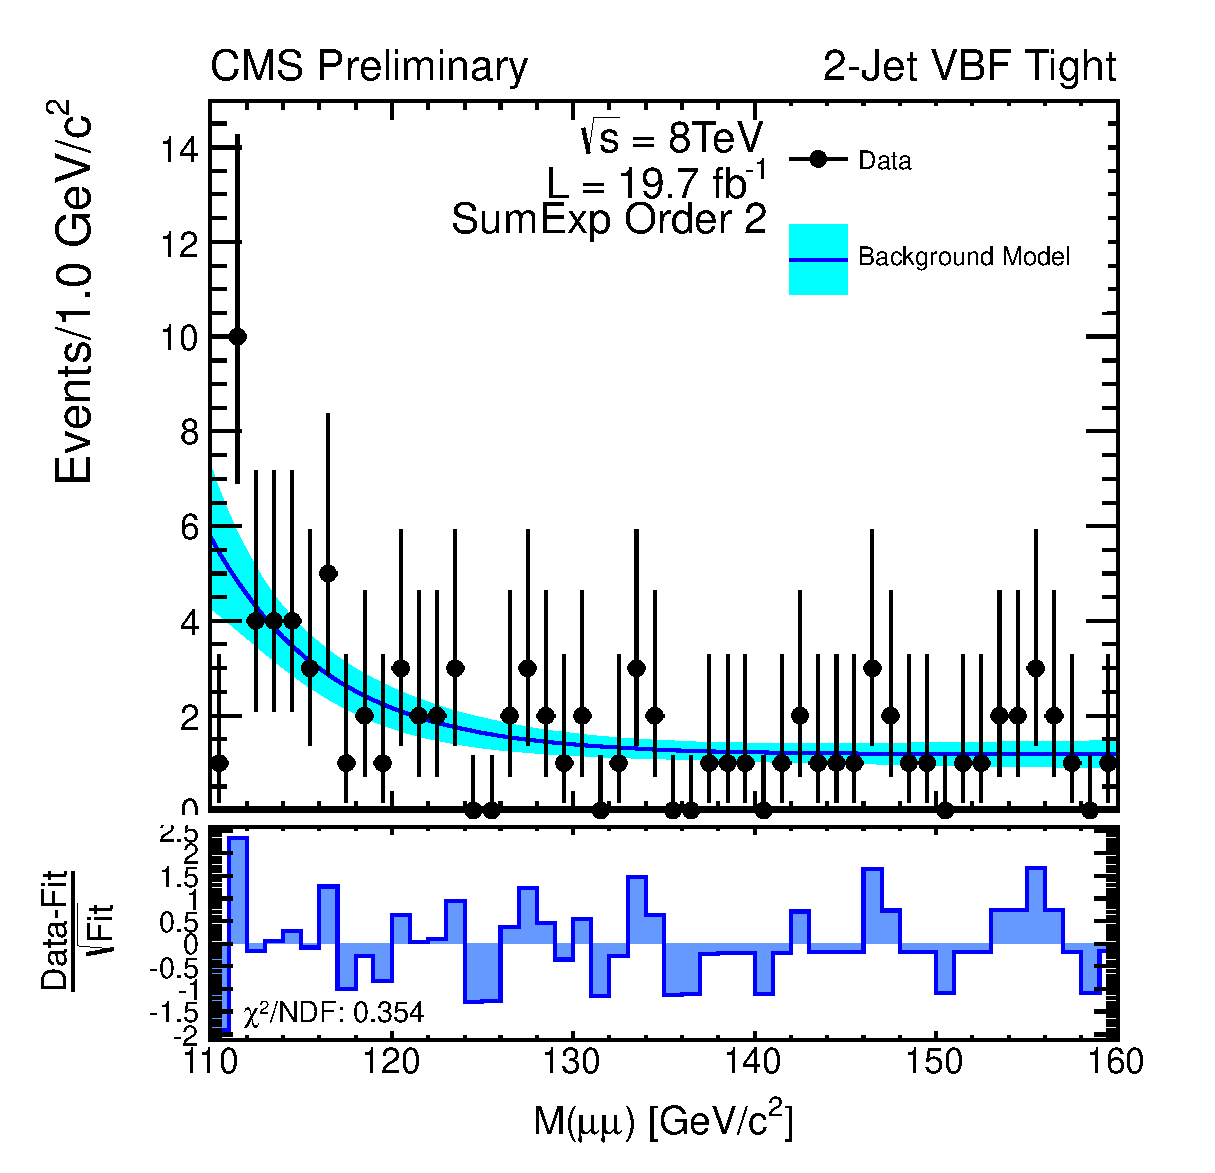
\includegraphics[height=55mm]{wholeRangeHggStudy1/plotsOrderStudyExpPow/order_Shape_Jet2CutsVBFPass_SumExp2}
      \end{center}
  \end{columns}
  \begin{center}
  \end{center}
\end{frame}

\begin{frame}
\frametitle{Bernstein 0,1-Jet Tight BO}
  \begin{columns}[c]
   \column{60mm}
      \begin{center}
      \tiny
\begin{tabular}{|l|c|c|c|c|} \hline
Order & Goodness & $-\ln\mathcal{L}$ & $-2\ln\lambda$ & $p_{\chi^2}$ \\ 
 & of Fit  &  & &  \\ \hline \hline
1 & 0 & -89577.79 & 1266.13 & 2.59e-277  \\ \hline
2 & 4.43e-40 & -88944.72 & 222.67 & 2.37e-50  \\ \hline
3 & 0.00147 & -88833.39 & 21.74 & 3.12e-06  \\ \hline
4 & 0.079 & -88822.52 & 17.11 & 3.53e-05  \\ \hline
5 & 0.579 & -88813.97 & 8.08 & 0.00447  \\ \hline
\bf 6 & \bf 0.796 & \bf -88809.92 & \bf 1.84 & \bf 0.175  \\ \hline
7 & 0.785 & -88809.00 & -0.22 & 1  \\ \hline
8 & 0.732 & -88809.12 & 0.46 & 0.496  \\ \hline
9 & 0.72 & -88808.88 & - & -  \\ \hline
\end{tabular}
\\
\normalsize
\vspace{2em}
\bf
      \end{center}
   \column{60mm}
      \begin{center}
        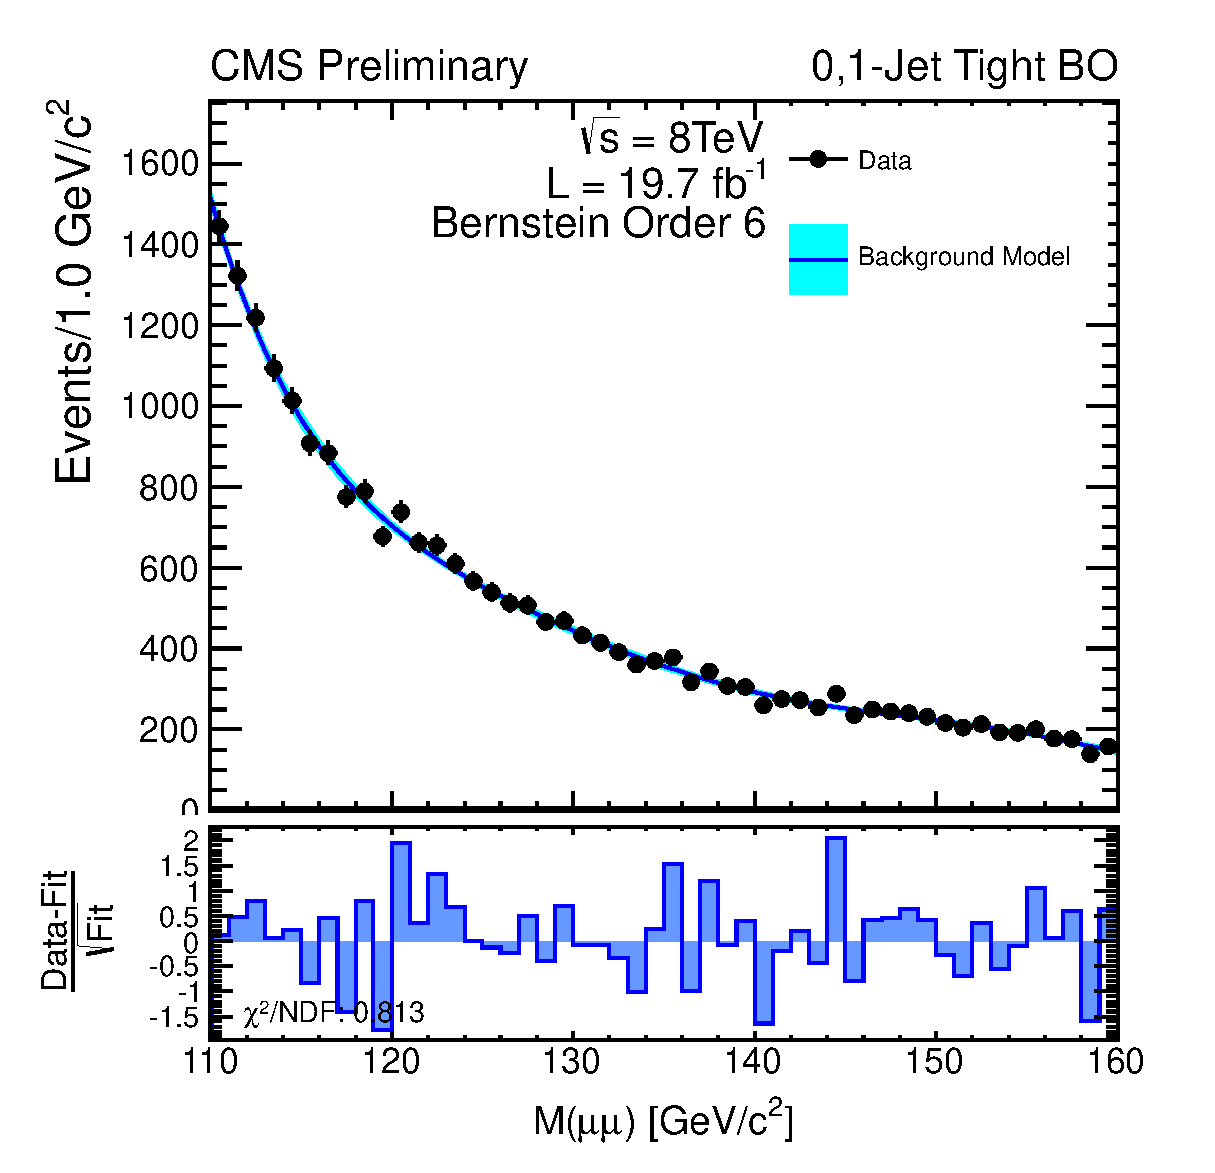
\includegraphics[height=55mm]{wholeRangeHggStudy1/plotsOrderStudyPolysHighOrders/order_Shape_Jets01PassPtG10BO_Bernstein6}
      \end{center}
  \end{columns}
  \begin{center}
  \end{center}
\end{frame}



\begin{frame}
\frametitle{Bernstein 0,1-Jet Tight BE}
  \begin{columns}[c]
   \column{60mm}
      \begin{center}
      \tiny
\begin{tabular}{|l|c|c|c|c|} \hline
Order & Goodness & $-\ln\mathcal{L}$ & $-2\ln\lambda$ & $p_{\chi^2}$ \\ 
 & of Fit  &  & &  \\ \hline \hline
1 & 8.86e-130 & -40641.90 & 550.30 & 1.08e-121  \\ \hline
2 & 2.93e-14 & -40366.75 & 78.28 & 8.96e-19  \\ \hline
3 & 0.000671 & -40327.61 & 14.38 & 0.000149  \\ \hline
4 & 0.0137 & -40320.42 & 7.27 & 0.007  \\ \hline
\bf 5 & \bf 0.0359 & \bf -40316.78 & \bf 0.40 & \bf 0.526  \\ \hline
6 & 0.0299 & -40316.58 & 1.72 & 0.19  \\ \hline
7 & 0.0286 & -40315.73 & - & -  \\ \hline
\end{tabular}
\\
\normalsize
\vspace{2em}
\bf
      \end{center}
   \column{60mm}
      \begin{center}
        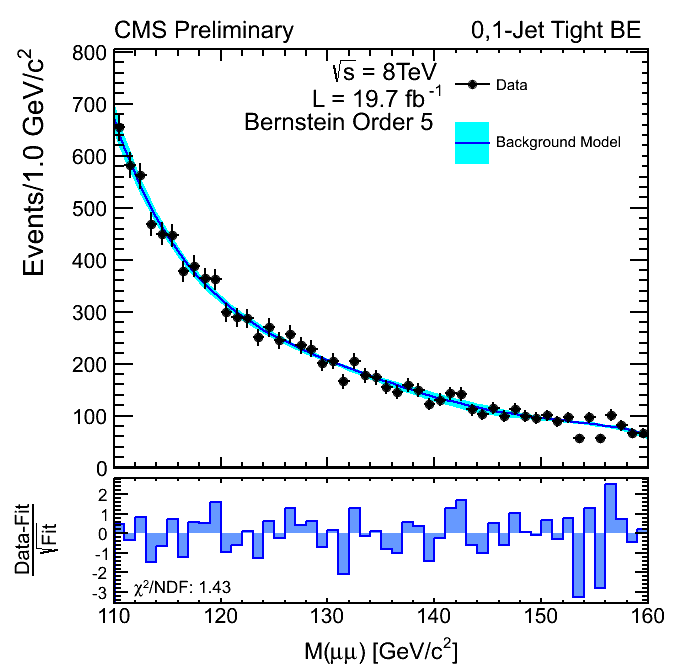
\includegraphics[height=55mm]{wholeRangeHggStudy1/plotsOrderStudyPolysHighOrders/order_Shape_Jets01PassPtG10BE_Bernstein5}
      \end{center}
  \end{columns}
  \begin{center}
  \end{center}
\end{frame}


\begin{frame}
\frametitle{Bernstein 2-Jet VBF Tight}
  \begin{columns}[c]
   \column{60mm}
      \begin{center}
      \tiny
\begin{tabular}{|l|c|c|c|c|} \hline
Order & Goodness & $-\ln\mathcal{L}$ & $-2\ln\lambda$ & $p_{\chi^2}$ \\ 
 & of Fit  &  & &  \\ \hline \hline
1 & 0.226 & -346.05 & 7.90 & 0.00495  \\ \hline
\bf 2 & \bf 0.648 & \bf -342.10 & \bf 2.36 & \bf 0.124  \\ \hline
3 & 0.729 & -340.92 & 1.33 & 0.248  \\ \hline
4 & 0.724 & -340.25 & 0.49 & 0.484  \\ \hline
5 & 0.675 & -340.01 & 0.60 & 0.439  \\ \hline
6 & 0.67 & -339.71 & 0.53 & 0.465  \\ \hline
7 & 0.624 & -339.44 & 0.38 & 0.537  \\ \hline
8 & 0.582 & -339.25 & 0.26 & 0.609  \\ \hline
9 & 0.531 & -339.12 & - & -  \\ \hline
\end{tabular}
\\
\normalsize
\vspace{2em}
\bf
Upturn at High Mass Will Be Difficult for Other Functions to Fit
\\
Not-Physical Behavior
      \end{center}
   \column{60mm}
      \begin{center}
        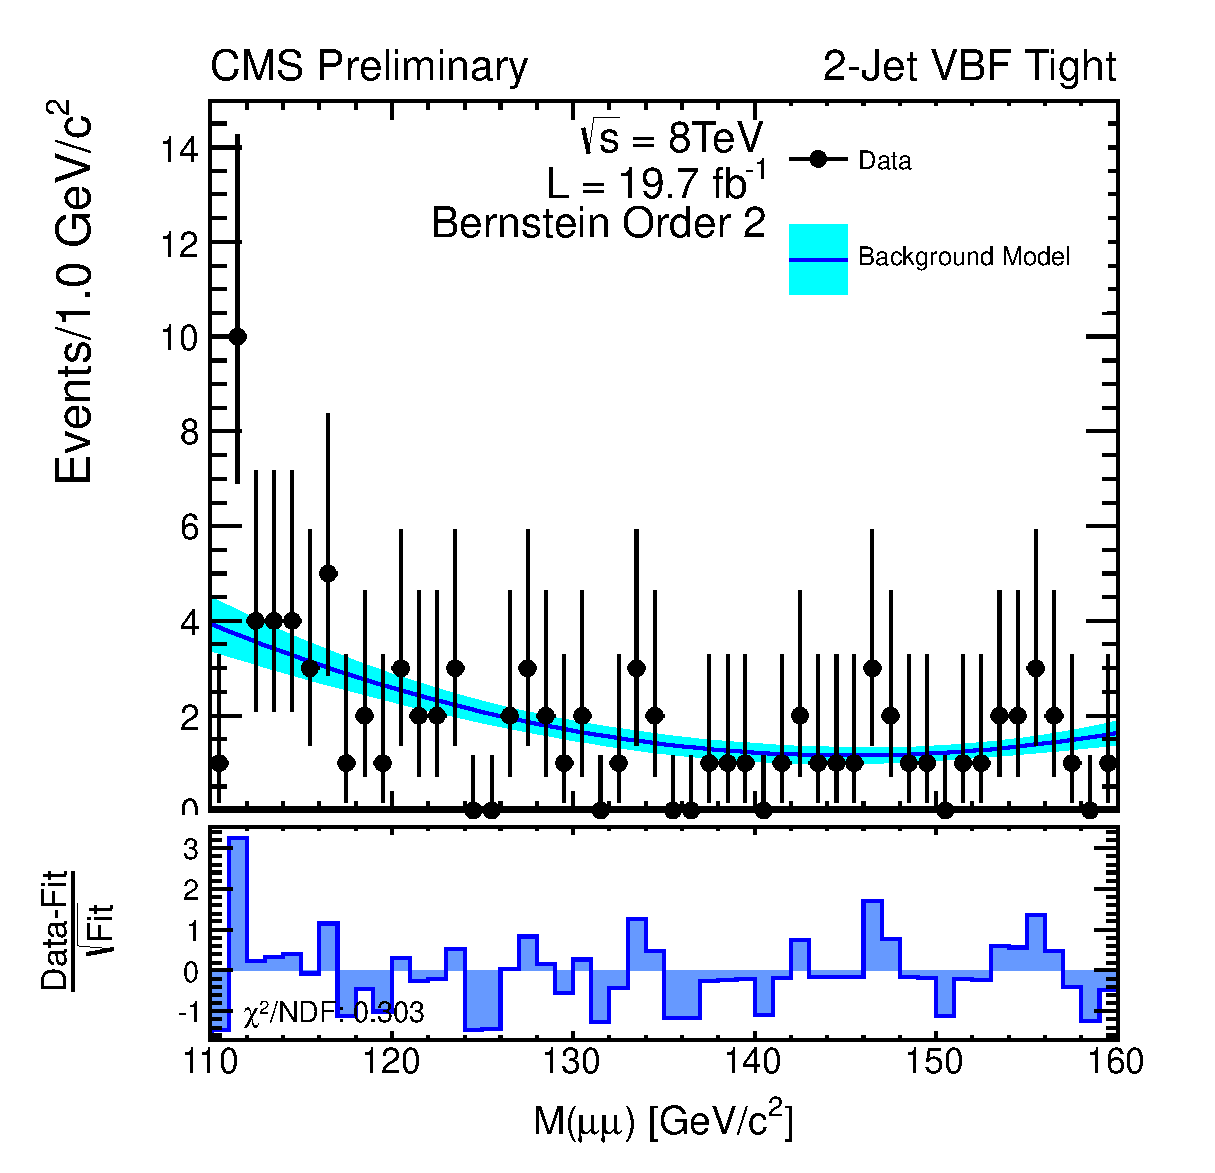
\includegraphics[height=55mm]{wholeRangeHggStudy1/plotsOrderStudyPolysLowOrders/order_Shape_Jet2CutsVBFPass_Bernstein2}
      \end{center}
  \end{columns}
  \begin{center}
  \end{center}
\end{frame}

\begin{frame}
\frametitle{Bernstein 2-Jet GF Tight}
  \begin{columns}[c]
   \column{60mm}
      \begin{center}
      \tiny
\begin{tabular}{|l|c|c|c|c|} \hline
Order & Goodness & $-\ln\mathcal{L}$ & $-2\ln\lambda$ & $p_{\chi^2}$ \\ 
 & of Fit  &  & &  \\ \hline \hline
1 & 0.00793 & -2478.49 & 14.63 & 0.000131  \\ \hline
2 & 0.101 & -2471.17 & 13.08 & 0.000299  \\ \hline
\bf 3 & \bf 0.496 & \bf -2464.63 & \bf 1.86 & \bf 0.172  \\ \hline
4 & 0.558 & -2463.70 & 0.20 & 0.656  \\ \hline
5 & 0.531 & -2463.60 & 0.34 & 0.558  \\ \hline
6 & 0.502 & -2463.43 & 0.39 & 0.535  \\ \hline
7 & 0.473 & -2463.24 & 0.98 & 0.322  \\ \hline
8 & 0.464 & -2462.75 & 0.33 & 0.568  \\ \hline
9 & 0.433 & -2462.59 & - & -  \\ \hline
\end{tabular}
\\
\normalsize
\vspace{2em}
\bf
Very Large Fit Errors
      \end{center}
   \column{60mm}
      \begin{center}
        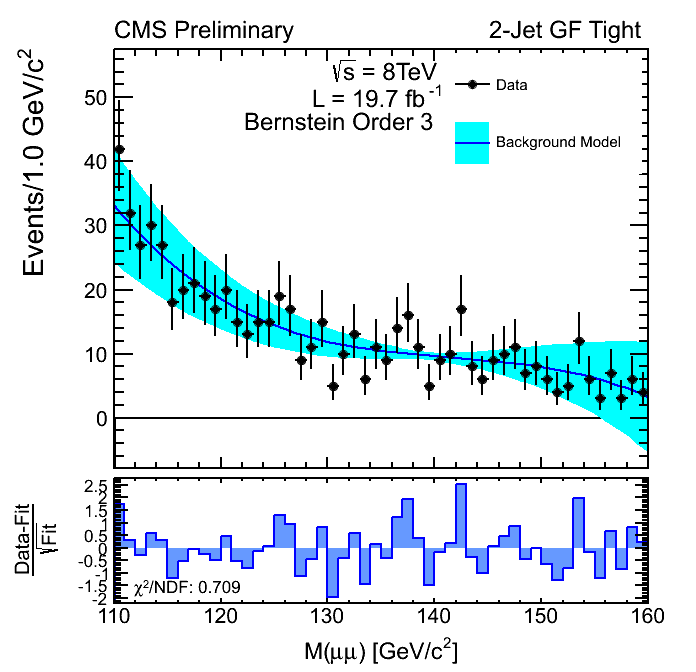
\includegraphics[height=55mm]{redoWholeRange/orderBernstein/order_Shape_Jet2CutsGFPass_Bernstein3}
      \end{center}
  \end{columns}
  \begin{center}
  \end{center}
\end{frame}


\begin{frame}
\frametitle{Bernstein 2-Jet Loose}
  \begin{columns}[c]
   \column{60mm}
      \begin{center}
      \tiny
\begin{tabular}{|l|c|c|c|c|} \hline
Order & Goodness & $-\ln\mathcal{L}$ & $-2\ln\lambda$ & $p_{\chi^2}$ \\ 
 & of Fit  &  & &  \\ \hline \hline
1 & 1.75e-17 & -14072.56 & 127.93 & 1.16e-29  \\ \hline
2 & 0.466 & -14008.60 & 7.46 & 0.00631  \\ \hline
3 & 0.698 & -14004.87 & 4.84 & 0.0278  \\ \hline
\bf 4 & \bf 0.849 & \bf -14002.45 & \bf 1.80 & \bf 0.179  \\ \hline
5 & 0.851 & -14001.54 & 0.85 & 0.356  \\ \hline
6 & 0.859 & -14001.12 & 0.43 & 0.512  \\ \hline
7 & 0.845 & -14000.90 & 1.55 & 0.213  \\ \hline
8 & 0.849 & -14000.13 & 1.26 & 0.262  \\ \hline
9 & 0.833 & -13999.50 & - & -  \\ \hline
\end{tabular}
\\
\normalsize
\vspace{2em}
\bf
      \end{center}
   \column{60mm}
      \begin{center}
        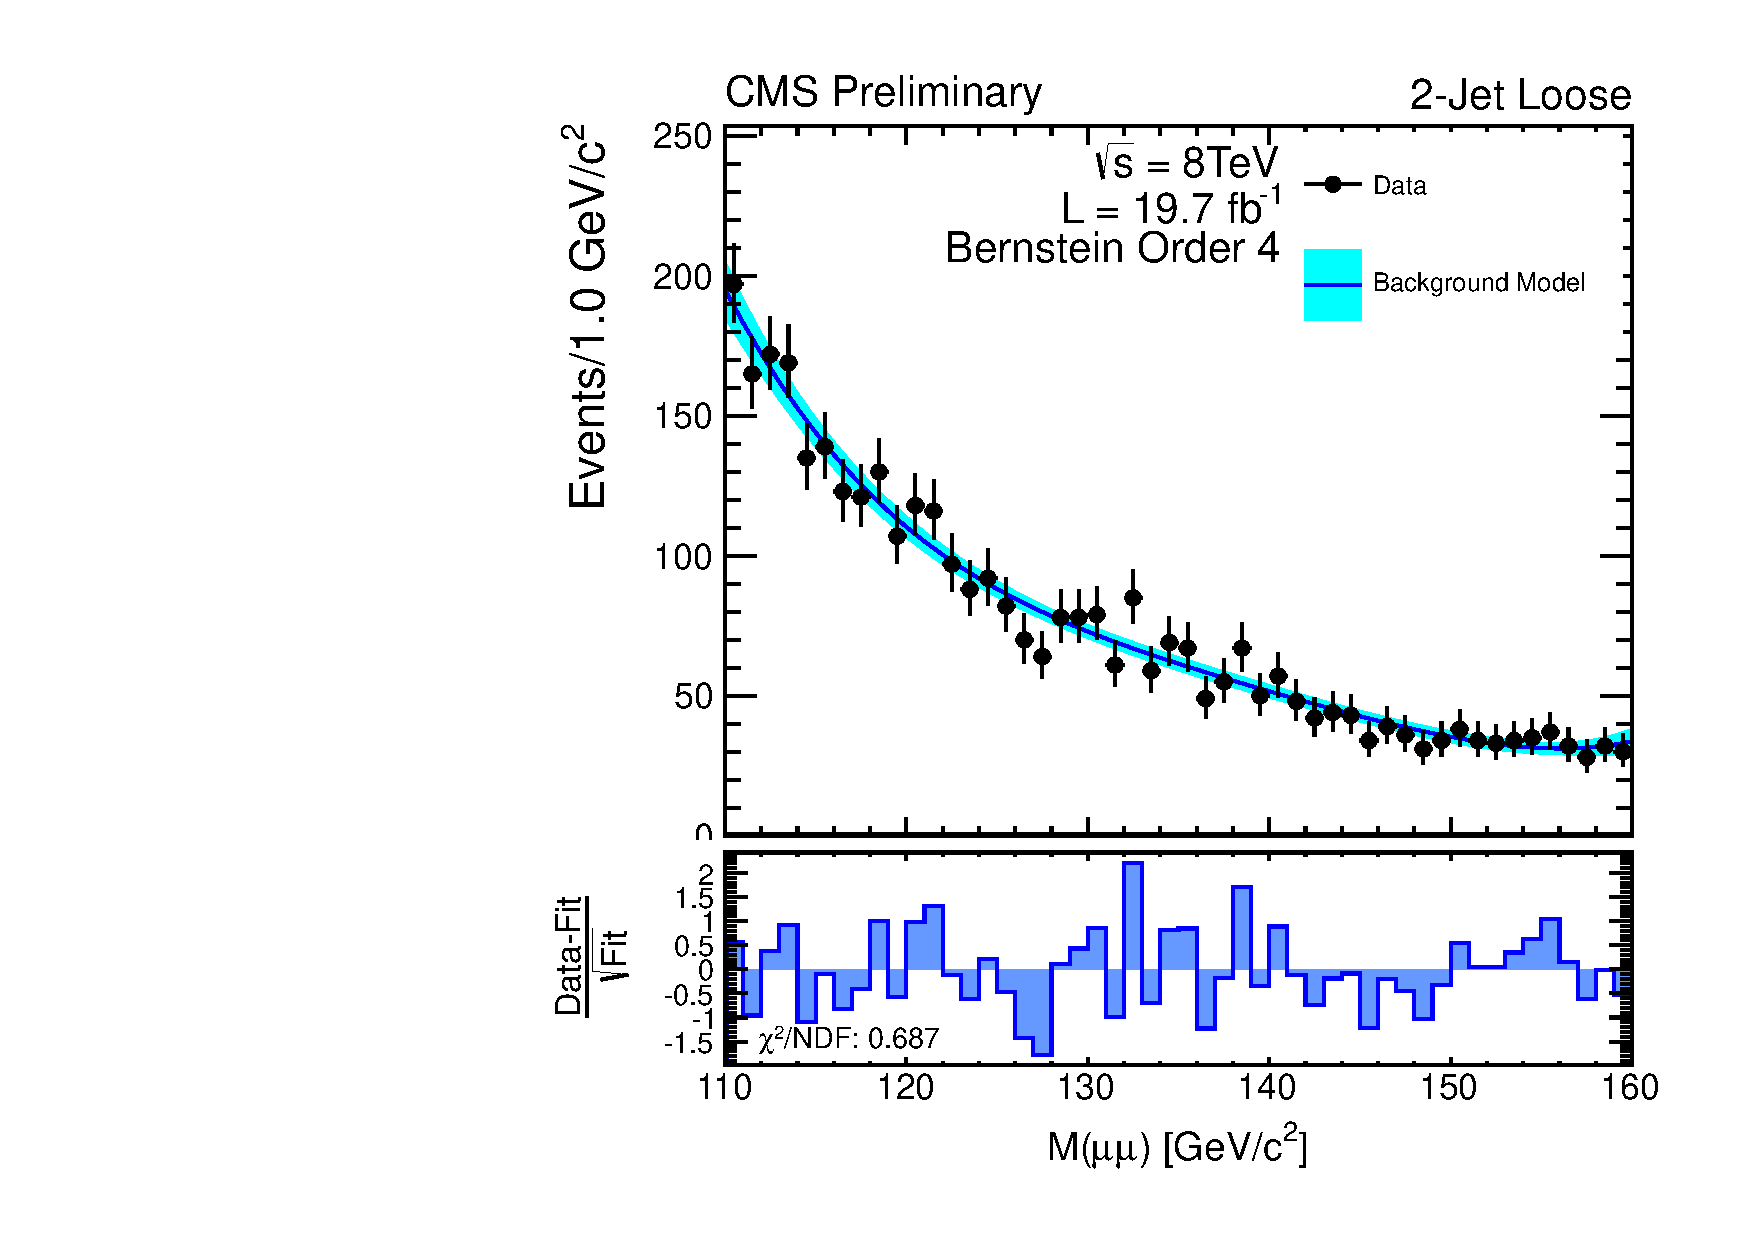
\includegraphics[height=55mm]{wholeRangeHggStudy1/plotsOrderStudyPolysLowOrders/order_Shape_Jet2CutsFailVBFGF_Bernstein4.pdf}
      \end{center}
  \end{columns}
  \begin{center}
  \end{center}
\end{frame}


\begin{frame}
\frametitle{Chebyshev Fits: 0,1-Jets Loose BB}
\vspace{-1em}
\begin{columns}[c]
 \column{60mm}
    \begin{center}
      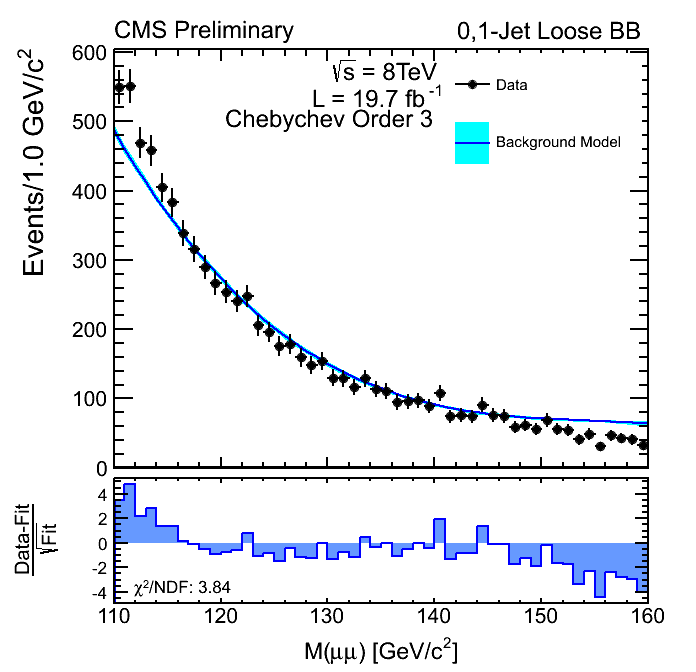
\includegraphics[height=55mm]{2013-10-04SystematicBiasStudy1/order_Shape_Jets01FailPtG10BB_Chebychev3}
    \end{center}
 \column{60mm}
    \begin{center}
      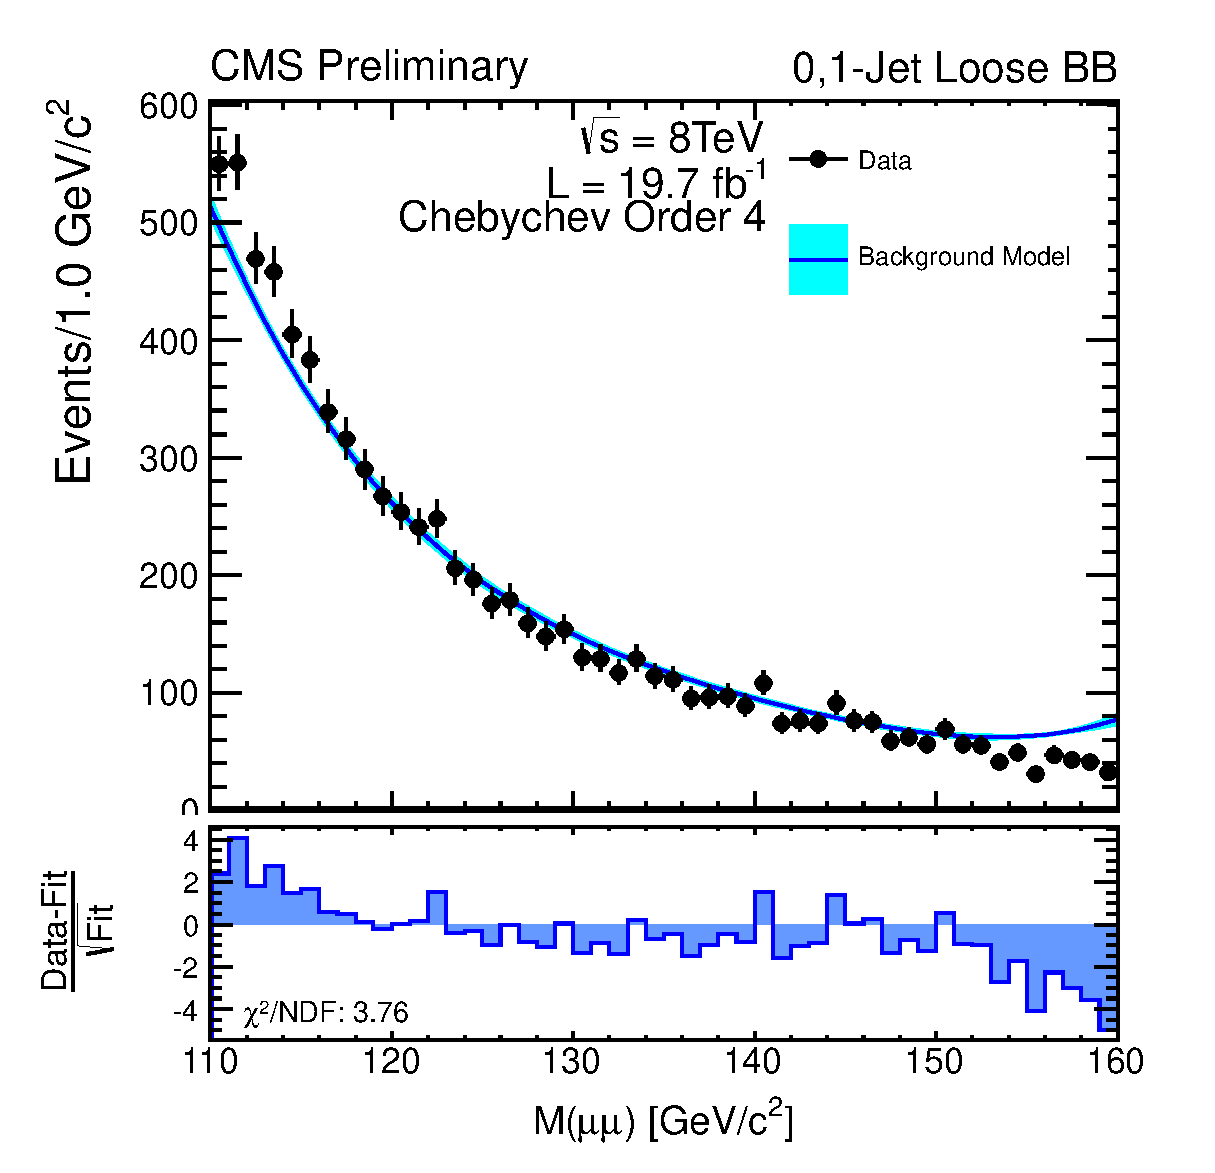
\includegraphics[height=55mm]{2013-10-04SystematicBiasStudy1/order_Shape_Jets01FailPtG10BB_Chebychev4}
    \end{center}
\end{columns}
\begin{center}
\bf
Some Feature of 0,1-Jet Loose Categories Messes Up Chebyshev Fits Near Boundaries
\\
\textcolor{red}{Won't Investigate Chebyshev Further}

\end{center}
\end{frame}

\begin{frame}
\frametitle{Sum of Powers Fits: 0,1-Jets Tight BB}
\begin{columns}[c]
 \column{60mm}
    \begin{center}
      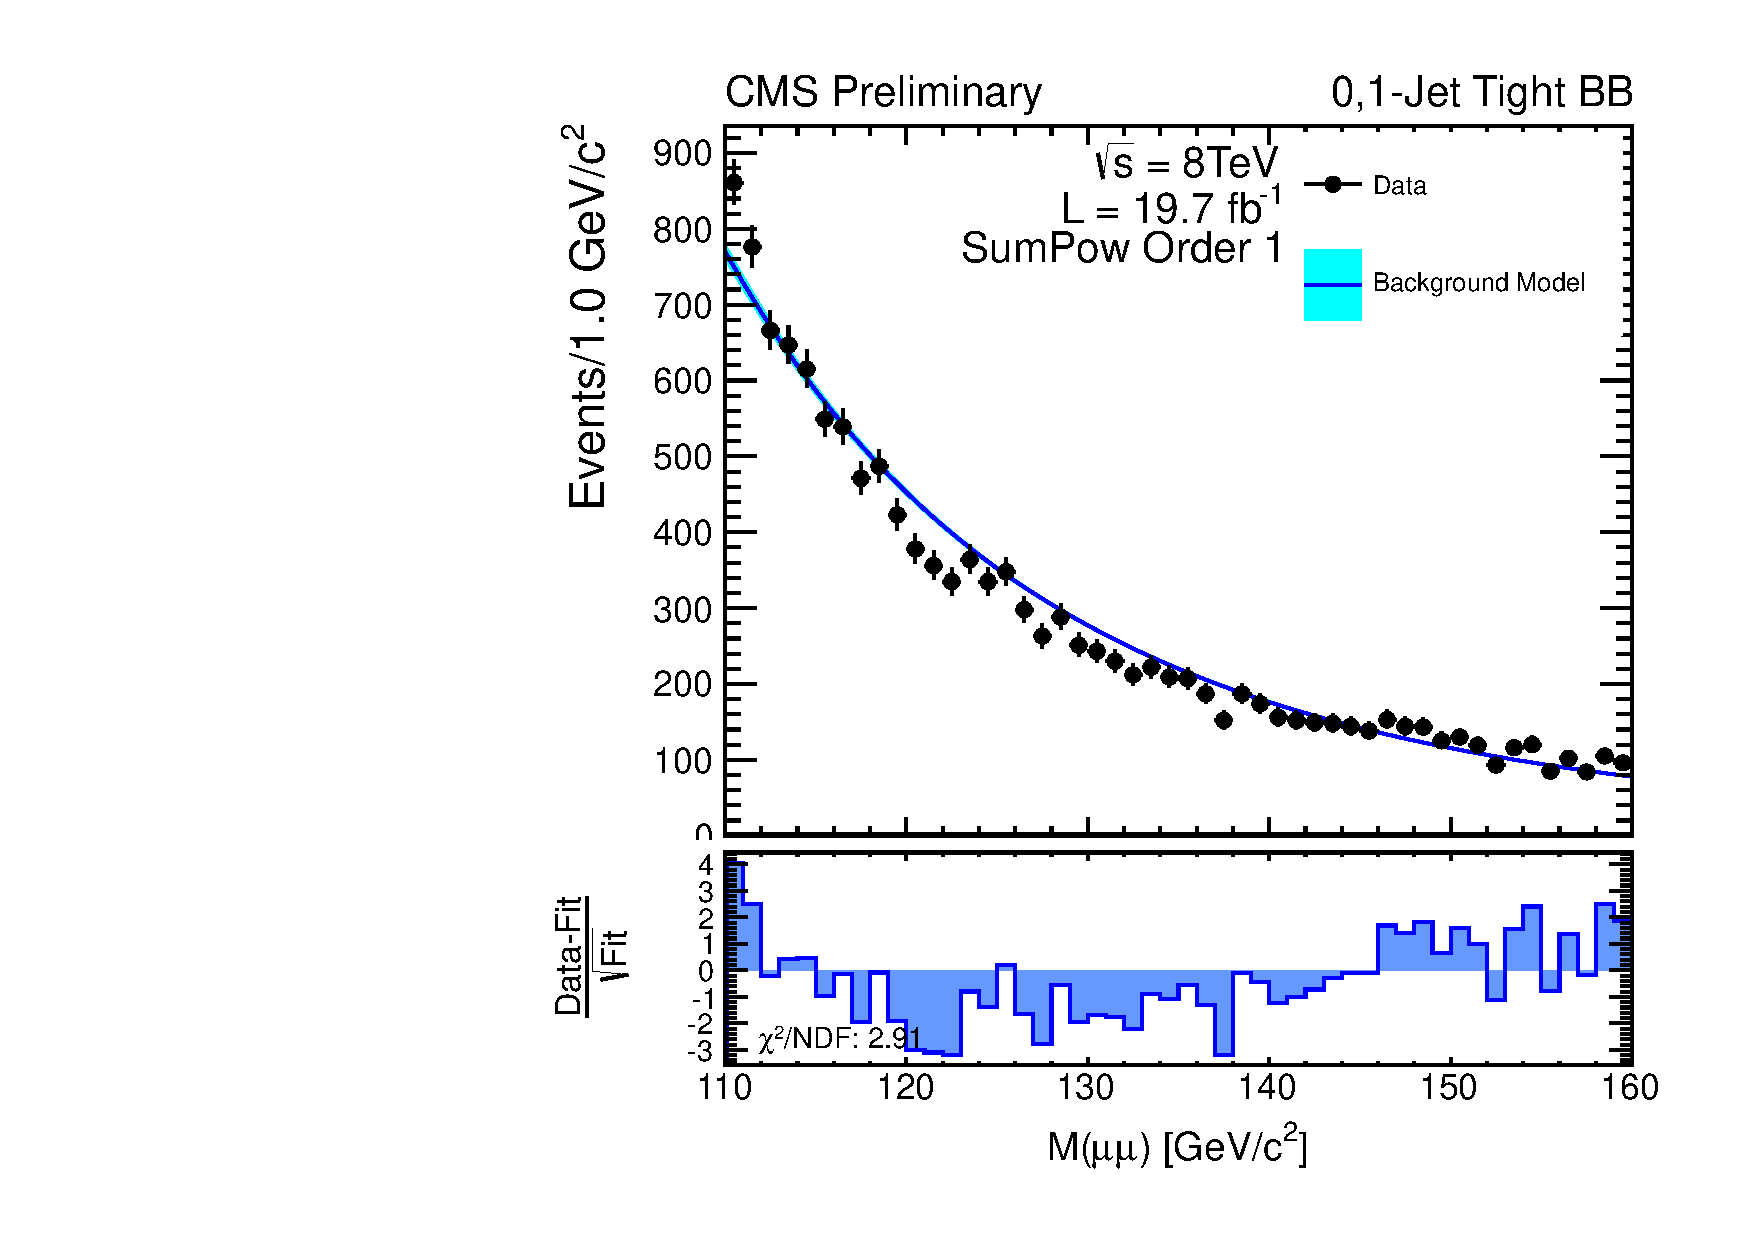
\includegraphics[height=55mm]{2013-10-04SystematicBiasStudy1/order_Shape_Jets01PassPtG10BB_SumPow1}
    \end{center}
 \column{60mm}
    \begin{center}
      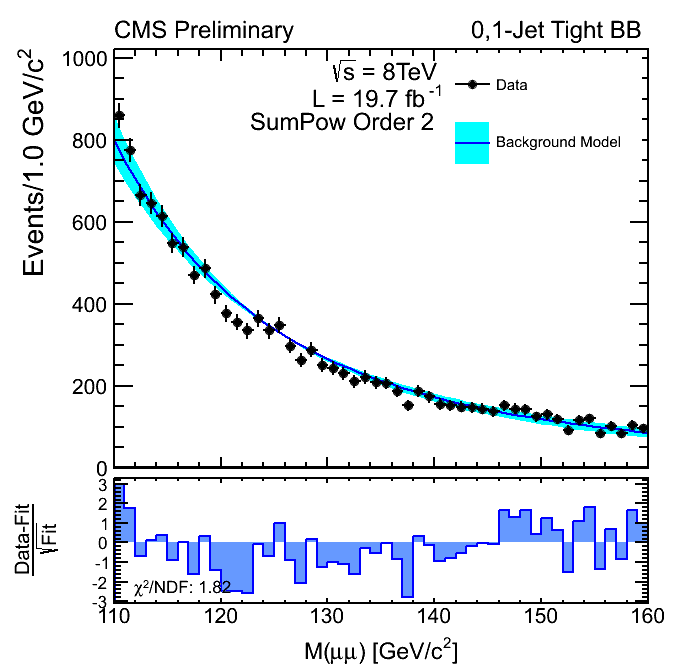
\includegraphics[height=55mm]{2013-10-04SystematicBiasStudy1/order_Shape_Jets01PassPtG10BB_SumPow2}
    \end{center}
\end{columns}
\begin{center}
\bf
Doesn't Seem To Describe Shape Well
\\
Other 0,1-Jet Categories \& Higher Orders Similar
\end{center}
\end{frame}

\begin{frame}
\frametitle{Example Bias w.r.t. Bernstein Reference}
  \vspace{-1ex}
  \begin{center}
    Bias for $m_H=125\GeVcc{}$
    \\ \vspace{0.5ex}
    \scriptsize
    \begin{tabular}{|l|c|c|c|} \hline
%  Bernstein  Bias per category for mh =  125
Category                  & Bias ($\sigma/\sigma_{SM}$) & Uncertainty  ($\sigma/\sigma_{SM}$) & Bias/Uncertainty \\ \hline \hline
0,1-Jet Tight BB         &       -0.1 &        7.1 &      -0.01 \\ \hline
0,1-Jet Tight BO         &        0.0 &        7.4 &       0.00 \\ \hline
0,1-Jet Tight BE         &       -1.6 &       14.8 &      -0.11 \\ \hline
0,1-Jet Tight OO         &        0.0 &       13.0 &       0.00 \\ \hline
0,1-Jet Tight OE         &        0.1 &       18.0 &       0.01 \\ \hline
0,1-Jet Tight EE         &        8.4 &       46.0 &       0.18 \\ \hline
0,1-Jet Loose BB         &        1.0 &       26.4 &       0.04 \\ \hline
0,1-Jet Loose BO         &        2.0 &       27.7 &       0.07 \\ \hline
0,1-Jet Loose BE         &        0.1 &       54.8 &       0.00 \\ \hline
0,1-Jet Loose OO         &        3.5 &       53.6 &       0.07 \\ \hline
0,1-Jet Loose OE         &        3.9 &       71.6 &       0.05 \\ \hline
0,1-Jet Loose EE         &       26.7 &      176.5 &       0.15 \\ \hline
2-Jet VBF Tight          &        0.0 &        5.1 &       0.00 \\ \hline
2-Jet GF Tight           &        2.6 &       14.7 &       0.18 \\ \hline
2-Jet Loose              &        0.2 &       13.6 &       0.01 \\ \hline
    \end{tabular}
\\
  \small
  \end{center}
\end{frame}

\begin{frame}
\frametitle{Example Bias w.r.t. Sum of Exponentials Reference}
  \vspace{-1ex}
  \begin{center}
    Bias for $m_H=125\GeVcc{}$
    \\ \vspace{0.5ex}
    \scriptsize
    \begin{tabular}{|l|c|c|c|} \hline
%  SumExp  Bias per category for mh =  125
Category                  & Bias ($\sigma/\sigma_{SM}$) & Uncertainty  ($\sigma/\sigma_{SM}$) & Bias/Uncertainty \\ \hline \hline
0,1-Jet Tight BB         &        1.6 &        7.1 &       0.22 \\ \hline
0,1-Jet Tight BO         &        0.7 &        7.5 &       0.09 \\ \hline
0,1-Jet Tight BE         &        2.4 &       14.8 &       0.16 \\ \hline
0,1-Jet Tight OO         &        2.1 &       13.0 &       0.16 \\ \hline
0,1-Jet Tight OE         &        1.2 &       18.0 &       0.07 \\ \hline
0,1-Jet Tight EE         &        9.0 &       45.9 &       0.20 \\ \hline
0,1-Jet Loose BB         &        5.8 &       26.6 &       0.22 \\ \hline
0,1-Jet Loose BO         &        4.3 &       27.8 &       0.15 \\ \hline
0,1-Jet Loose BE         &        6.6 &       55.0 &       0.12 \\ \hline
0,1-Jet Loose OO         &        7.4 &       53.9 &       0.14 \\ \hline
0,1-Jet Loose OE         &        9.4 &       71.6 &       0.13 \\ \hline
0,1-Jet Loose EE         &       20.9 &      178.2 &       0.12 \\ \hline
2-Jet VBF Tight          &       -0.4 &        5.3 &      -0.08 \\ \hline
2-Jet GF Tight           &        3.6 &       14.5 &       0.25 \\ \hline
2-Jet Loose              &       -1.2 &       13.7 &      -0.09 \\ \hline
    \end{tabular}
\\
  \small
  \end{center}
\end{frame}


\end{document}
